\documentclass[oneside,14pt]{book}

\usepackage[T1,T2A]{fontenc}
\usepackage[utf8]{inputenc}
\usepackage[english,russian]{babel}
\usepackage{indentfirst}

%\usepackage[paperwidth=15cm,paperheight=7.5cm]{geometry} % планшет
%\usepackage[paperwidth=297mm,paperheight=210mm]{geometry} % A4
%\usepackage[paperwidth=148mm,paperheight=105mm]{geometry} % A5
\usepackage[paperwidth=18cm,paperheight=13cm,margin=5mm]{geometry} % экран*2

%\usepackage[colorlinks=true,
%]{hyperref}
%\newcommand{\email}[2]{#1\ \href{mailto:#2}{<\nolinkurl{#2}>}}
% %\newcommand{\email}[2]{\emph{#1\ <#2>}}
\usepackage[unicode,colorlinks,
pdftitle={Azbuka ARMaturschika (ru)},
pdfauthor={(c) Dmitry Ponyatov <dponyatov@gmail.com>, SSAU ASCL},
pdfsubject={ru manual on writing programs for Cortex-M MCUs},
pdfkeywords={ARM} {Cortex} {MCU} {ARMatura} {Arduino} {SSAU}
]{hyperref}

\usepackage{wrapfig}
\usepackage{graphicx}
\usepackage{epstopdf}
\DeclareGraphicsExtensions{.eps}

\usepackage{listings}
\usepackage{dirtree}
\usepackage[usenames,dvipsnames,svgnames]{xcolor}
\newcommand{\cppcolor}{\color[rgb]{0.94, 0.97, 1.0}} % Alice blue
\newcommand{\asmcolor}{\color[rgb]{0.98, 0.92, 0.84}} % Antique white
\newcommand{\ldcolor}{\color[rgb]{0.67, 0.9, 0.93}} % Blizzard Blue
\newcommand{\concolor}{\color[rgb]{0.88, 1.0, 1.0}} % Light cyan
\newcommand{\makecolor}{\color[rgb]{0.9, 0.9, 0.98}} % Lavender mist

%\definecolor{cppcolor}{rgb}{0.94, 0.97, 1.0}
\lstset{frame=single,
numbers=left, numberstyle=\small, numbersep=1mm,
tabsize=4,
keywordstyle=\color{blue}\texttt,
commentstyle=\color{cyan}\texttt,
inputencoding=utf8, extendedchars=true, showspaces=false,  
inputencoding=cp1251
}
\usepackage{lstlangarm}
\usepackage{lstlanggnumake}
\usepackage{lstlanggnuld}
\usepackage{lstlanggnudump}

\lstdefinestyle{cpp}{language=C++,backgroundcolor=\cppcolor}
\lstdefinestyle{asm}{language={[ARM]Assembler},backgroundcolor=\asmcolor}
\lstdefinestyle{gnuld}{language={[GNU]Link},backgroundcolor=\ldcolor}
\lstdefinestyle{con}{backgroundcolor=\concolor}
\lstdefinestyle{mk}{language=[GNU]Make,backgroundcolor=\makecolor}
\lstdefinestyle{objdump}{language=[GNU]Dump}

\newcommand{\cm}[1]{Cortex-M#1}
\newcommand{\cx}{\cm{x}}

\newcommand{\vld}{STM32VLDISCOVERY}

%\renewcommand{\url}[1]{\textbf{#1}}
\newcommand{\email}[1]{$<$\href{mailto:#1}{\textbf{#1}}$>$}

\newcommand{\cpp}{$C^{+^{+}}$}

\newcommand{\cp}[1]{\footnote{копипаста: #1}}

\newcommand{\thmod}{Thumb}
\newcommand{\armod}{ARM}
\newcommand{\arm}{ARM}

\newcommand{\Reg}[1]{\textbf{#1}}
\newcommand{\R}[1]{\Reg{R#1}}

\newcommand{\periph}[1]{\texttt{#1}}
\newcommand{\jtag}{\periph{JTAG}}

\usepackage{wasysym} % smileys
\usepackage{gensymb} % celsius
\usepackage{amssymb} % windows key
\usepackage{textcomp} % bigcircle

\usepackage[os=win]{menukeys}
\newcommand{\winstart}{$\boxplus$}
\newcommand{\file}[1]{\textbf{\textsf{#1}}}
\newcommand{\window}[1]{\textbf{\textit{#1}}}
\newcommand{\alarm}[1]{{\color{DarkRed}#1}}
\newcommand{\wcmd}[1]{\keys{\winstart+R}\ \directory{#1}}
\newcommand{\checkbox}{$\boxtimes$}
\newcommand{\uncheckbox}{$\square$}
\newcommand{\lms}{\keys{$\lhd$}}
\newcommand{\rms}{\keys{$\rhd$}}
\newcommand{\eclpx}{\window{Project Explorer}}

\newcommand{\win}[1]{
\includegraphics[height=10ex]{fig/winlogo.jpg} #1}
\newcommand{\lin}[1]{
\includegraphics[height=10ex]{fig/linuxcolor.png} #1}
\newcommand{\bug}{
\includegraphics[height=10ex]{fig/iconbug.png}}

\newcommand{\linux}{Linux}
\newcommand{\git}{Git}
\newcommand{\eclipse}{\textcircled{$\equiv$}\textsc{eclipse}}
%\newcommand{\term}[1]{\underline{#1}}
\newcommand{\term}[1]{\underline{\color{DarkBlue} #1}}
\newcommand{\miktex}{MiK\TeX}
\newcommand{\internet}{Internet}
\newcommand{\ql}{Quantum$^{\circledR}L^{e}aPs$}
\newcommand{\gdb}{GDB}

\newcommand{\make}{\file{make}}
\newcommand{\makefile}{\file{Makefile}}

\usepackage{tocloft}
\newcommand{\listlabname}{Лабораторные работы}
\newlistof{lab}{ex}{\listlabname}
\newcommand{\labpart}[1]{\addcontentsline{ex}{part}{#1}}
\newcounter{labworkcounter}
\newcommand{\labwork}[1]{
\refstepcounter{labworkcounter}
\section*{ЛР\thelabworkcounter: #1}
\addcontentsline{toc}{subsection}{ЛР\thelabworkcounter: #1}
\addcontentsline{ex}{section}{ЛР\thelabworkcounter: #1}
}
\newcommand{\labref}[1]{ЛР\ref{#1}}

\newcommand{\thetitle}{Азбука халтурщика-ARMатурщика}

\newcommand{\mytitle}[1]{
\title{\Huge{\thetitle}\\
#1\\
\normalsize{учебный курс по микроконтроллерам \cx:\\
Миландр 1986ВЕ, STM32F, LPC21xx}}
}

\author{(copypasta) Понятов Д.А. \email{dponyatov@gmail.com}, ИКП СГАУ}


\setdoclang{ru}{russian} % toggle comment to set en/ru mode
\begin{document}

\mytitle{\ }
\maketitle
\tableofcontents
\listoflab

\secru{Рабочая среда разработчика встраиваемых систем}
	
\begin{itemize}
  \item Операционная система с набором типовых утилит
  
  Для Windows требуется дополнительно установить несколько модулей из пакета
  \file{GnuWin32}, чтобы обеспечить минимальную совместимость с UNIX-средой.
  Установка \file{GnuWin32}\ описана в \labref{winsoftinstall}.
  
  Установка Linux описана в \labref{debianinstall}.
  
  \item Система управления версиями (\term{VCS})
  
  VCS предназначены для хранения полной истории изменений файлов проекта, и
  позволяют получить выгрузку проекта на любой момент времени, вести несколько
  веток разработки, получить историю изменений конкретного файла, или сравнить
  две версии файла (\term{diff}).
  
  Установка VCS \git\ описана в \labref{gitinstall}.
  
  \item Текстовый редактор или интегрированная среда разработки (IDE)
  
  Редактирование текстов программ и скриптов сборки (компиляции) с
  цветовой подсветкой синтаксиса (в зависимости от языка файла),
  \term{автодополнением}\ и вызовом программ-утилит нажатием сочетаний 
  клавиш. Также включает различные вспомогательные функции, например
  отладочный интерфейс и отображение объектов программ.
  
  Установка IDE \eclipse\ описана в \labref{eclipseinstall}.
  
  \item Тулчайн
  
  Пакет кросс-компилятора, ассемблера, линкера и других утилит типа make,
  objdump,.. для получения прошивок из исходных текстов программ.
  
  Установка GNU toolchain описана в \labref{gnuinstall}.
  
  \item ПО для программатора, JTAG-адаптера
  
  Загрузка полученной прошивки в целевое устройство, редактирование памяти, 
  внутрисхемная отладка в процессе работы устройства, прямое измение сигналов на
  выводах процессора (граничное сканирование и тестирование железа).
  
  Установка ПО для адаптеров ST-Link \labref{stlinkinst}, Segger J-Link
  \labref{jlinkinst}.
  
  \item Симулятор для отладки программ без железа
  
  Симулятор может использоваться как ограниченная замена реального железа
  для начального обучения, и для отладки программ, не завязанных на работу
  железа.
  
  Установка QEMU \labref{qemuinstall}.
  
  \item Система верстки документации
  
  Для документирования проектов и написания руководств нужна система верстки
  документации, выполняющая трансляцию текстов программ и файлов 
  документации в выходной формат, чаще всего \file{.pdf} и \file{.html}.
  
  Установка \LaTeX\ \labref{texinstall}.
  
\end{itemize}


	\secdown
	\secru{САПР электронных устройств}
		\secdown
		\secru{САПР EDA KiCAD}

\cp{http://ru.wikibooks.org/wiki/KiCad}

KiCad\ --- распространяемый по лицензии GNU GPL программный комплекс класса EDA
с открытыми исходными текстами, предназначенный для разработки электрических схем и печатных плат.

Кроссплатформенность компонентов KiCad обеспечивается использованием 
библиотеки wxWidgets. Поддерживаются операционные системы Linux, 
Windows NT 5.x, FreeBSD и Solaris.

Разработчик\ --- Жан-Пьер Шарра (фр. Jean-Pierre Charras), исследователь 
в LIS (фр. Laboratoire des Images et des Signaux — Лаборатория Изображений 
и Сигналов) и преподаватель электроники и обработки изображений в фр. 
IUT de Saint Martin d’Hères (Франция).

\bigskip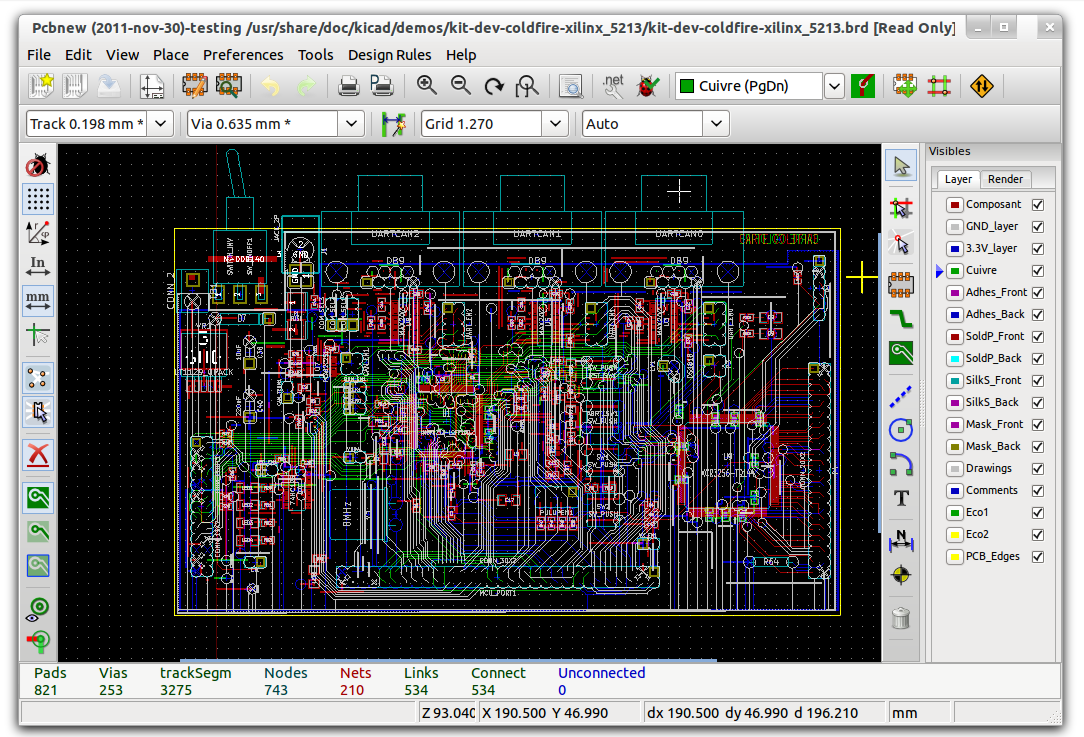
\includegraphics[height=0.5\textheight]{kicad/kicad_pcbnew.png}


		\secup
 	%
  Компилятор преобразует программы на языке программирования в \term{объектный
  код} (смесь кусочков машинного кода со служебной информацией) или в
  текст на языке ассемблера.
  
  \term{Кросс-компилятор}\ (arm-none-eabi-gcc) отличается от обычного
  компилятора тем, что генерирует код не для компьютера на котором он выполняется
  (\term{хост-система}, \verb|$HOST|), а для компьютера другой
  архитектуры\ --- \term{целевой} системы, \verb|$TARGET|.
  
  \term{Ассемблер}\ (as) преобразует человекочитаемый код программы в объектный
  код.
  
  \term{Линкер}\ (ld) объединяет несколько файлов объектного кода в один,
  и корректирует машинный код с учетом его конечного размещения в памяти
  целевой системы (адреса переменных, адреса переходов, размещение сегментов
  кода и данных в физической памяти целевой системы).
  
  \term{Дампер}\ (objdump) преобразует сегменты кода/данных из файла,
  полученного линкером, в формат, необходимый для ПО программатора: бинарные файлы, Intel
  HEX, ELF,.. загружаемые в масочное ПЗУ, FlashPROM (и EEPROM данных на МК
  ATmega).
  

	\secup

\secru{Установка ПО}
	\secdown
% 	\labwork{Установка Debian GNU/Linux}\label{debianinstall}


% 	\labwork{Установка Git}\label{gitinstall}

Создадим рабочий каталог, установим систему контроля версий \git\ref{git}\ и 
получим локальную копию проекта этой книги, содержащий кроме текста для издательской системы
\LaTeX\ еще и исходные коды библиотек, примеры кода и т.п., которые вы захотите
использовать в своих проектах.

\bigskip\wcmd{\url{http://git-scm.com/download/win}}

Запуститься закачка установочного пакета scm-git (\file{Git-1.9.4-preview20140611.exe}), после его загрузки
запустите установщик, 

\bigskip
\menu{Welcome>Next}

\bigskip
\menu{GNU GPL>Next} 

\bigskip
\menu{Select components>Windows Explorer Integration>Simple Context Menu>Git GUI here>Next}

\bigskip
\menu{Use Git and optional Unix tools from the Command Prompt>Next}

\bigskip
\menu{Use OpenSSH>Next}

\bigskip
\menu{Checkout Windows-style>Next}

\bigskip
\menu{Extracting files...}

\bigskip
\menu{Completing Setup>\uncheckbox\ View ReleaseNotes>Finish}

\bigskip
Проверим что \git\ правильно установился:

\bigskip\wcmd{cmd}

\bigskip
\begin{lstlisting}[style=con]
C:\Documents and Settings\pda>git --version
git version 1.9.4.msysgit.0
\end{lstlisting}

\bigskip
Первое, что вам следует сделать после установки \git а\ ---указать ваше имя и
адрес электронной почты. Это важно, потому что каждый коммит в \git е содержит
эту информацию, и она включена в коммиты, передаваемые вами:
\begin{lstlisting}[style=con]
C:\Documents and Settings\pda>git config --global user.name "Vasya Pupkin"
C:\Documents and Settings\pda>git config --global user.email no@mail.com
C:\Documents and Settings\pda>git config --global push.default simple
\end{lstlisting}

\bigskip
Эти настройки достаточно сделать только один раз, поскольку в этом случае 
\git\ будет использовать эти данные для всего, что вы делаете.
 Если для каких-то отдельных проектов вы хотите указать другое имя или
электронную почту, можно выполнить эту же команду без параметра \verb|--global|
в каталоге с нужным проектом.

\bigskip
Создаем каталог \file{D:/ARM}\ и выгружаем текущую копию этой книги из
репозитория \url{https://github.com/ponyatov/CortexMx}, создавая
свой собственный локальный \term{репозиторий проекта}.

\bigskip\wcmd{cmd}

\bigskip
\begin{lstlisting}[style=con]
C:\Documents and Settings\pda>D:
D:\>mkdir \ARM
D:\>cd \ARM
D:\ARM>git clone --depth=1 https://github.com/ponyatov/CortexMx.git book
\end{lstlisting}

% 	\labwork{Установка GNU toolchain}\label{gnuchaininstall}


% 	\labwork{Установка утилит GnuWin32}\label{gnuwinstall}


% 	\labwork{Установка Java}\label{javainstall}

Для работы IDE \eclipse\ требуется установленная Java:

\bigskip\wcmd{\url{http://www.oracle.com/technetwork/java/javase/downloads/}}

\bigskip\begin{itemize}
  \item 
Минимальный вариант\ ---  ставим только Java Runtime:

\menu{Java Platform, Standard Edition>JRE>Download>Accept
License>\file{jre-8u5-windows-i586.exe}}

\menu{\file{jre-8u5-windows-i586.exe}>Welcome>\checkbox\ Change destination
folder>Install}

\menu{Destination folder>\file{D:/Java/jre8}>Next>Installing>Close}

  \item
Если вы планируете параллельно еще и осваивать язык Java\ --- ставим
Java SE JDK: 

\menu{Java Platform, Standard Edition>JDK>Download>Accept
License>\file{jdk-8u5-windows-i586.exe}}

\menu{\file{jdk-8u5-windows-i586.exe}>Welcome>Next}

\menu{Install to: \file{D:/Java/jdk8}>Next}

\menu{JRE Distination folder>Install to: \file{D:/Java/jre8}>Next}

\menu{Java SE Development Kit 8 Update 5 Successfully Installed>Close}

\end{itemize}


 	\labwork{Установка IDE \eclipse}\label{eclipseinstall}

\bigskip
Для работы IDE \eclipse\ требуется установленная Java \labref{javainstall}.

\bigskip
Для установки доступны два варианта:
\begin{enumerate}
\item \textbf{Eclipse Standard} базовый вариант среды, в ЛР рассмотрен именно он для иллюстрации 
ручной установки расширений
\item \textbf{Eclipse IDE for C/C++ Developers} вариант сборки 
уже включает расширение CDT, поэтому в следующий раз рекомендуем сразу качать его,
это упростит и съэкономит немного времени на установку рабочей среды
\end{enumerate}

\bigskip\wcmd{\url{http://www.eclipse.org/downloads/}}

\bigskip\menu{Eclipse Standard>Windows 32
Bit>Download>\file{eclipse-standard-luna-R-win32.zip}}

\bigskip Перетащите каталог \file{eclipse} из архива в \file{D:/ARM} и
создайте удобным для вас способом ссылку на \file{D:/ARM/eclipse/eclipse.exe}.

\bigskip
\includegraphics[height=0.3\textheight]{fig/EclipseSplash.png}

\bigskip Workspace\ --- рабочий каталог, в котором создаются каталоги отдельных
проектов, типа \file{D:/WORK}. Eclipse создаст в нем служебный каталог
\file{.metadata}, и поместит в него служебную информацию, относящуюся сразу ко
всем проектам. Как побочный эффект, если в workspace уже есть какой-то каталог,
можно создать новый проект (например \file{book}), и в левой части рабочей
области \eclipse\ в окне \window{Project Explorer}\ появится дерево файлов
\file{book/*}.

\bigskip\menu{\file{D:/ARM/eclipse/eclipse.exe}>Workspace>\file{D:/ARM}>Use as
default>OK}

\bigskip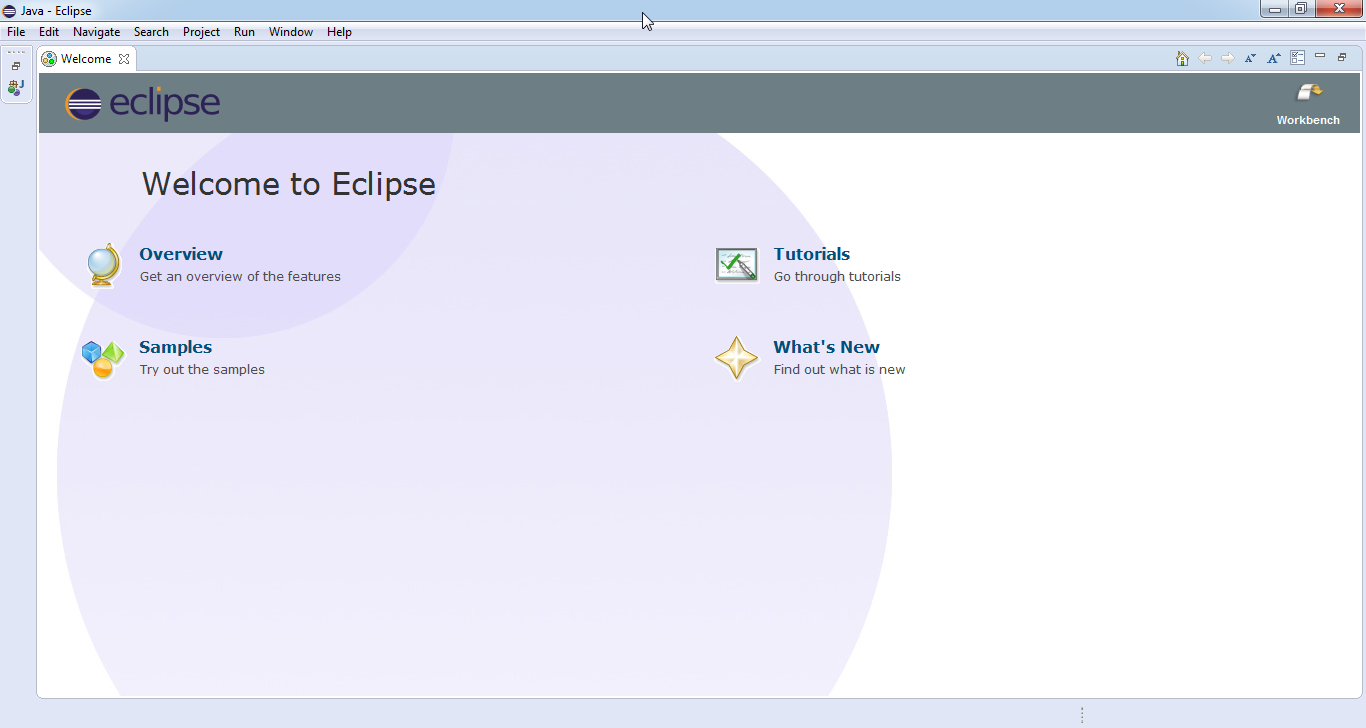
\includegraphics[width=0.9\textwidth]{fig/EclipseMain.png}

\bigskip Проверяем наличие обновлений

\bigskip\menu{Help>Check for Updates>Details>No updates found>OK}

\bigskip В базовом варианте Eclipse поддерживает только Java, поэтому нужно
установить расширение для работы с С/C++: \file{CDT}.

\bigskip
Проект \file{CDT}\ предоставляет полнофункциональную интегрированную среду
для разработки на Си и \cpp. Поддерживаются: управление проектами и
компиляцией для различных тулчейнов, стандартная сборка через
\file{make}, навигация по исходным текстам, различные инструменты для
работы с иходным текстом, такие как иерархия типов, граф вызовов, браузер
подключаемых файлов, браузер макроопределений, редактор кода с подсветкой
синтаксиса, сворачивание синтаксических структур (фолдинг) и гипертекстовая
навигация, рефакторинг и генерация кода, средства визуальной отладки,
включающие просмотр памяти, регистров и дизассемблер.

\bigskip\wcmd{\url{http://www.eclipse.org/cdt/downloads.php}}

\bigskip Выделить и скопировать в буфер обмена ссылку

\file{p2 software repository}:
\url{http://download.eclipse.org/tools/cdt/releases/8.4}.

\bigskip Добавляем сетевое хранилище пакетов для \eclipse:

\bigskip\menu{\eclipse>Help>Install New Software>Work with>Add}

\bigskip\menu{Name>CDT}

\menu{Location>http://download.eclipse.org/tools/cdt/releases/8.4}

\menu{OK}

\bigskip
Выбрать (если оно не выбралось само) хранилище \menu{Work with:>CDT},
и в дереве выбора пакетов выбрать:

\bigskip
\dirtree{%
.1 CDT.
.2 CDT Main Features.
.3 \checkbox\ C/C++ Development Tools.
.2 CDT Optional Features.
.3 \checkbox\ C/C++ C99 LR Parser.
.3 \checkbox\ C/C++ GCC Cross Compiler Support.
.3 \checkbox\ C/C++ GDB Hardware Debugging.
}

\bigskip
\menu{Next>Next>Licenses>Accept>Finish}

\bigskip После установки пакетов появится окно с запросом перезапуска \eclipse.

\bigskip Аналогично ставим плагин GNU ARM Eclipse:

\bigskip
\menu{Help>Install>Work with>Add}

\menu{Name>GNU ARM plugin}

\menu{Location>\url{http://sourceforge.net/projects/gnuarmeclipse/files/Eclipse/updates/}}

\dirtree{%}
.1 GNU ARM C/C++ Cross Development Tools.
.2 \checkbox\ Cross Compiler Support.
.2 \checkbox\ Generic Cortex-M Project Template.
.2 \checkbox\ STM32Fx Project Templates.
.2 \checkbox\ OpenOCD Debugging Support.
}

\menu{Warning: You install unsigned content>Ok}

\bigskip
В \eclipse\ есть так называемые \term{перспективы} (perspective)\ --- это
переключаемые режимы отображения рабочего набора окон, настроенные под тип
работы. По умолчанию запускается перспектива \window{Java}. Нас
интересует перспектива \window{C/C++}:

\bigskip\menu{Window>Open Perspective>Other>C/C++>Ok}

\bigskip Также перспективу можно переключить кнопкой на панели в правом верхнем
углу:

\bigskip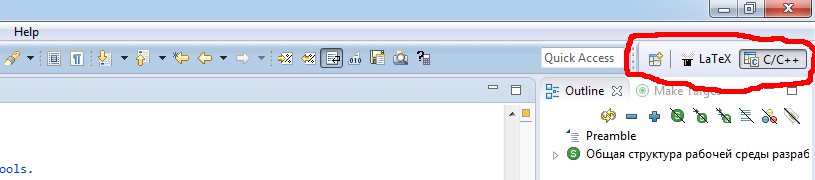
\includegraphics[width=0.9\textwidth]{fig/eclperpective.png}

\bigskip Для настройки привычных вам клавиш можно сразу зайти в
глобальные настроки среды и поменять привязку клавиш:

\bigskip\menu{Window>Preferences>General>Keys}

\menu{Type filter here:>F12}

\menu{Command}

\menu{Activate Editor>Binding>/удалить/}

\menu{Build Project>Binding>/нажать \keys{F12}/}

\menu{Apply>OK}



% 	\labwork{Установка симулятора QEMU}\label{qemuinstall}

Нередко в практике разработчика возникают ситуации, когда программное обеспечение (ПО) для микроконтроллера
приходится писать в отсутствии под рукой аппаратной платформы.

Например, печатная плата устройства отдана на подготовку к производству, а времени ждать
готовое устройство для тестирования на нем программного обеспечения нет.

В таких случаях для оценки работоспособности ПО можно воспользоваться программным симулятором целевого микроконтроллера.

Для интегрированной среды разработки \eclipse\ CDT в качестве программного
симулятора микроконтроллеров ARM можно использовать симулятор (или виртуальную машину,если быть точным) 
\file{qemu-arm} с интерфейсом командной строки:

\bigskip\menu{\wcmd{\url{http://qemu.weilnetz.de/w32/}}>\file{qemu-w32-setup-20140702.exe}}

\menu{\file{qemu-w32-setup-20140702.exe}>Welcome>Next>License>Agree}

\menu{Choose Components}

\dirtree{%
.1 QEMU.
.2 \uncheckbox\ System Emulations.
.3 \checkbox\ arm.
.3 \checkbox\ armw.
}

\menu{Next}

\menu{Destination Folder>\file{D:/ARM/qemu}>Next>Finish}

\bigskip Добавьте \file{D:/ARM/qemu}\ в системную переменную
\file{\$PATH}\ (\labref{winpath}).

\bigskip

\begin{lstlisting}[style=con]
C:\Documents and Settings\pda>qemu-system-arm -version
C:\Documents and Settings\pda>cat D:\ARM\qemu\stdout.txt
QEMU emulator version 2.0.90, Copyright (c) 2003-2008 Fabrice Bellard
\end{lstlisting}


% 	\labwork{Установка ПО ST-Link для \vld}\label{labinststsoft}

\menu{\wcmd{\url{http://www.google.com}}>ST-Link>ST-Link - STMicroelectronics}

\bigskip
\begin{tabular}{l l l}
\menu{STSW-LINK002>Download}	&ST-LINK USB driver for Windows XP&драйвер\\
\menu{STSW-LINK004>Download}	&STM32 ST-LINK utility&ПО программатора\\
\end{tabular}

\bigskip
\menu{\file{st-link\_usbdriver.zip}>\file{ST-Link\_USBdriver.exe}}

\menu{STLinkDriver>Welcome>Next>Install
to>\file{C:/ARM/STM32/STdriver}>Next>Install>Finish}

\bigskip
\menu{\file{stsw-link004.zip}>\file{STM32 ST-LINK Utility\_v3.4.0.exe}}

\menu{ST-LINK
Utility>Next>License>Yes>Distination>\file{C:/ARM/STM32/STLinkUtil}>Finish}

\menu{(сам запустился) Device Driver Install Wizard>Далее>Установить}

\bigskip
\menu{\winstart>STMicroelectronics>ST-LINK Utility>STM32 ST-Link}

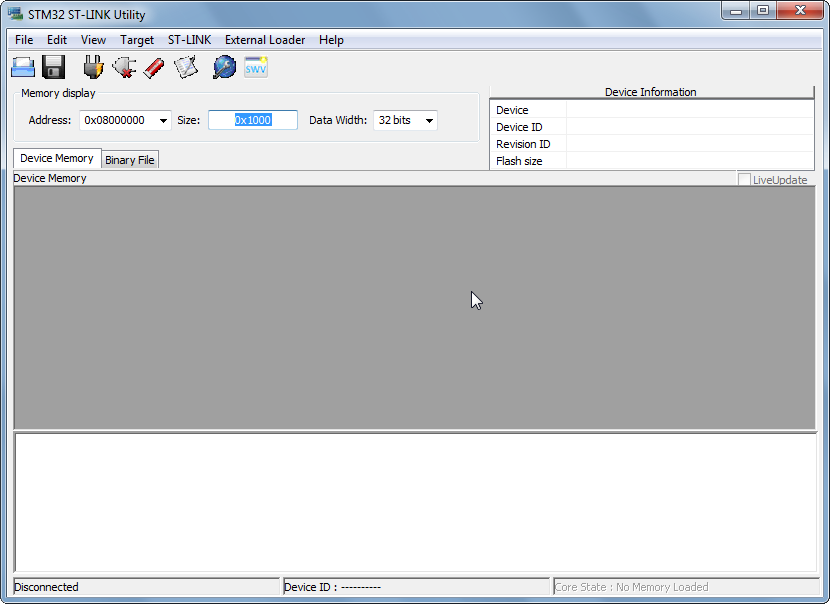
\includegraphics[height=0.5\textheight]{fig/stlink0.png}

\bigskip
\menu{STutil>Target>Connect}

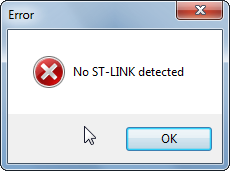
\includegraphics[height=0.2\textheight]{fig/nostlink.png}

\bigskip
Подключаем плату \vld\ кабелем, в системе подключается новое устройство,
на плате запускается ранее залитая в МК прошивка:

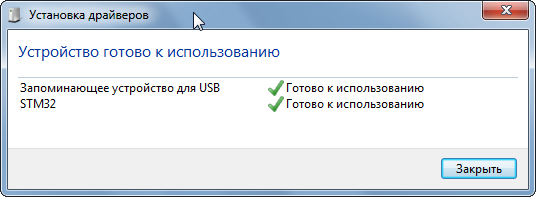
\includegraphics[height=0.3\textheight]{fig/stdrvok.png}

\bigskip
\menu{STutil>Target>Connect}

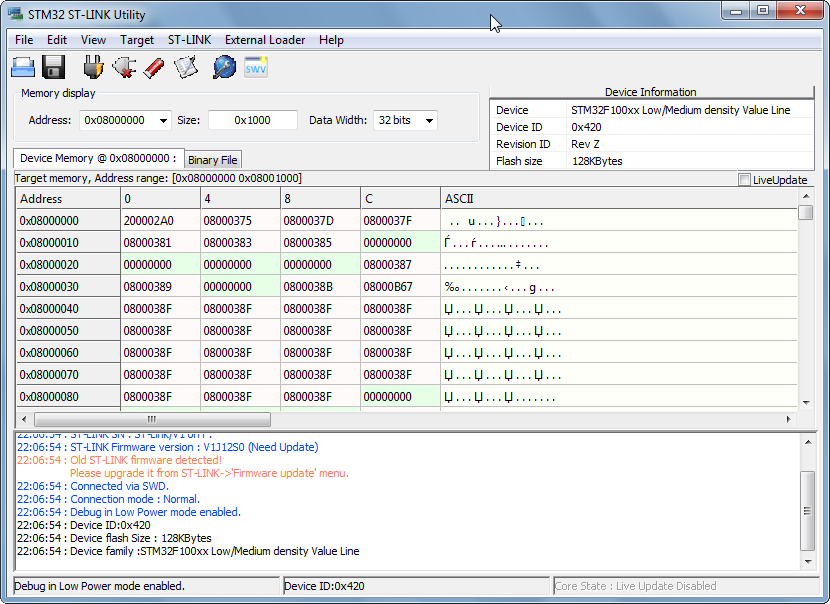
\includegraphics[width=0.9\textwidth]{fig/stconnected.png}

\bigskip
Обновление прошивки ST-Link:

\menu{ST Link>ST-LINK>Firmware update>Device Connect>not in DFU
mode}

\menu{передергиваем плату>Device connect>Upgrade to V.1.J13.S0>Yes}

\bigskip



% 	\labwork{Установка системы верстки документации \LaTeX}\label{texinstall}

Если вы планируете писать полноценную документацию на программы
и оборудование, или участовать в доделке этой книги, вы можете установить
систему верстки \LaTeX.

Для работы с \TeX\ требуется довольно приличное по усилиям
(само)обучение \cite{lvovsky}, но оно оправдывается если вы часто 
пишете документацию, особенно если в ней больше 10 формул.
Готовить документацию в M\$\ Word\ --- (само)убийство мозга и времени,
идеология подстановочных макросов \TeX, богатый набор доп.пакетов
и командный ввод формул очень доставляют.

\win{Скачайте и установите пакет \miktex:}

\bigskip\wcmd{\url{http://miktex.org/download}>Other Downloads>Net Installer}

\menu{Save as:>\file{D:/ARM/soft/MikTeX/miktex-netsetup-2.9.4503}}

\bigskip Загрузка дистрибутивных файлов

\menu{\file{miktex-netsetup-2.9.4503}>License>Accept>Далее}

\menu{Task>Download>Далее}

Если у вас постоянное internet-соединение: \menu{Package Set>Basic MiKTeX>Далее}

Для offline работы\footnote{когда неизвестно какие пакеты понадобятся\ ---
\miktex\ умеет их докачивать по необходимости} \menu{Package
Set>Complete MikTeX>Далее}

\menu{Download Source>Russian Federation (ctan.uni-altai.ru)>Далее}

\menu{Distribution
Directory>\file{D:/ARM/soft/MikTeX}>Далее>Start>Executing>Далее>Close}

\bigskip Установка из ранее загруженного дистрибутива

\menu{\file{D:/ARM/soft/MikTeX/miktex-\alarm{netsetup}-2.9.4503}>License>Accept>Далее}

\menu{Task>Install>Далее>Basic MiKTeX>Далее}

\menu{Install for>Anyone/Only for user>Далее}

\menu{Install \alarm{from}:>\file{D:/ARM/soft/MikTeX}>Далее}

\menu{Install to:>\file{D:/LaTeX/MiKTeX}>Далее}

\menu{Settings}

\menu{Preferred paper>A4}

Важная опция: автоматическая докачка отсутствующих пакетов
\alarm{\menu{Install missing packages>Yes}}

\menu{Далее>Start>Executing>Close}

\bigskip Двухступенчатая установка позволяет сначала скачать полный дистрибутив
\miktex, а затем установить его на другой компьютер, не подключенный к
\internet, или c медленным/платным каналом не дающим взять и качнуть 200 Мб.

\bigskip Для удобной работы с \file{.tex} файлами в \eclipse\ нужно поставить 
дополнение \file{TeXlipse}:

\bigskip
\menu{\eclipse>Help>Install>Work with>Add}

\menu{Name>TeXlipse}

\menu{Location>\url{http://texlipse.sourceforge.net}}

\dirtree{%}
.1 TeXlipse.
.2 \checkbox\ TeXlipse.
}

% 	\secru{ПО для JTAG-адаптера}


	\labwork{Установка KiCAD}\label{kicadinstall}

\bigskip
\menu{\wcmd{\url{http://www.kicad-pcb.org/}}>Download>KiCAD for OS }

\bigskip\menu{\file{KiCad\_stable-2013.07.07-BZR4022\_Win\_full\_version.exe}}

\bigskip

\menu{Installer Language>Russian>Ok}

\menu{Установка KiCAD 2013.07.07>Далее}

\menu{Лицензия>Принимаю}

\menu{Компоненты>\checkbox\ все>Далее}

\menu{Папка установки>\file{C:/Program Files/KiCad}>Установить}

\menu{Копирование файлов}

\menu{Завершение установки>\checked\ Wings3D>Готово}

\bigskip

\wcmd{\url{http://www.wings3d.com/}}


	\secup

\secru{IDE \eclipse}



\labwork{Установка IDE \eclipse}\label{eclipseinstall}

\bigskip
Для работы IDE \eclipse\ требуется установленная Java \labref{javainstall}.

\bigskip
Для установки доступны два варианта:
\begin{enumerate}
\item \textbf{Eclipse Standard} базовый вариант среды, в ЛР рассмотрен именно он для иллюстрации 
ручной установки расширений
\item \textbf{Eclipse IDE for C/C++ Developers} вариант сборки 
уже включает расширение CDT, поэтому в следующий раз рекомендуем сразу качать его,
это упростит и съэкономит немного времени на установку рабочей среды
\end{enumerate}

\bigskip\wcmd{\url{http://www.eclipse.org/downloads/}}

\bigskip\menu{Eclipse Standard>Windows 32
Bit>Download>\file{eclipse-standard-luna-R-win32.zip}}

\bigskip Перетащите каталог \file{eclipse} из архива в \file{D:/ARM} и
создайте удобным для вас способом ссылку на \file{D:/ARM/eclipse/eclipse.exe}.

\bigskip
\includegraphics[height=0.3\textheight]{fig/EclipseSplash.png}

\bigskip Workspace\ --- рабочий каталог, в котором создаются каталоги отдельных
проектов, типа \file{D:/WORK}. Eclipse создаст в нем служебный каталог
\file{.metadata}, и поместит в него служебную информацию, относящуюся сразу ко
всем проектам. Как побочный эффект, если в workspace уже есть какой-то каталог,
можно создать новый проект (например \file{book}), и в левой части рабочей
области \eclipse\ в окне \window{Project Explorer}\ появится дерево файлов
\file{book/*}.

\bigskip\menu{\file{D:/ARM/eclipse/eclipse.exe}>Workspace>\file{D:/ARM}>Use as
default>OK}

\bigskip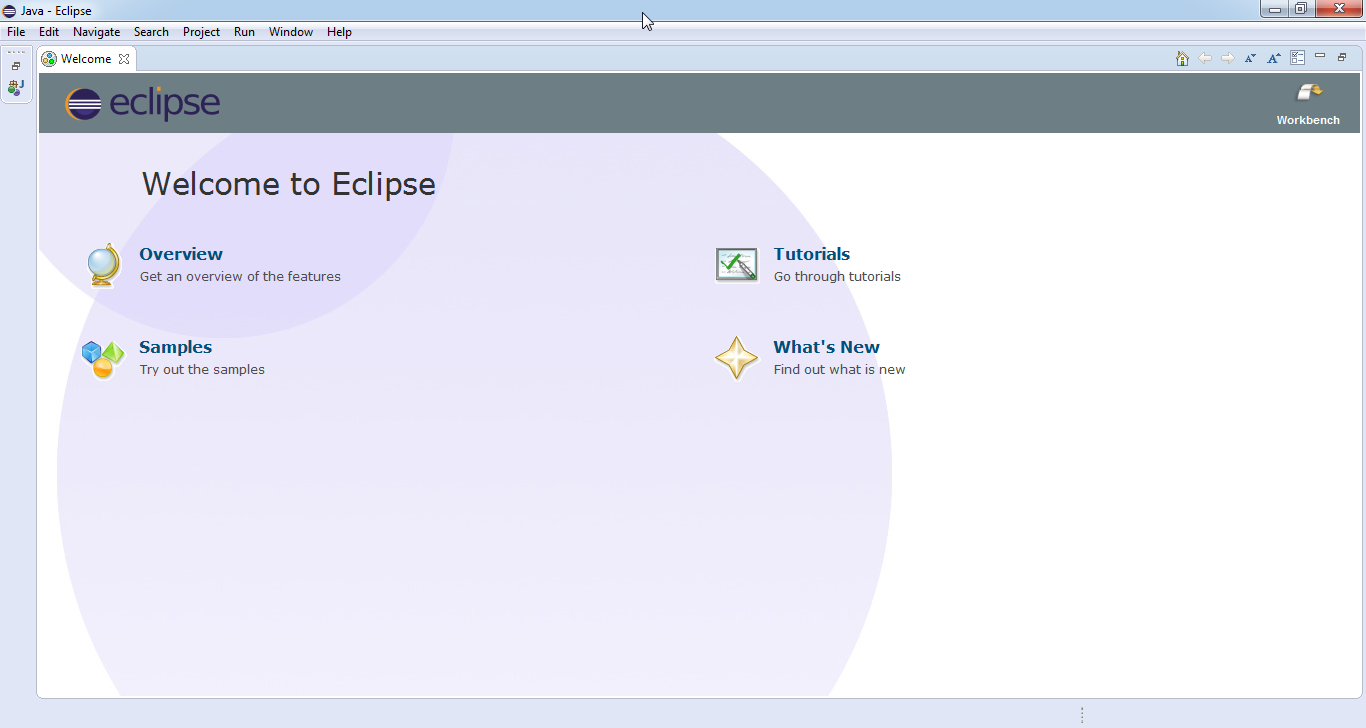
\includegraphics[width=0.9\textwidth]{fig/EclipseMain.png}

\bigskip Проверяем наличие обновлений

\bigskip\menu{Help>Check for Updates>Details>No updates found>OK}

\bigskip В базовом варианте Eclipse поддерживает только Java, поэтому нужно
установить расширение для работы с С/C++: \file{CDT}.

\bigskip
Проект \file{CDT}\ предоставляет полнофункциональную интегрированную среду
для разработки на Си и \cpp. Поддерживаются: управление проектами и
компиляцией для различных тулчейнов, стандартная сборка через
\file{make}, навигация по исходным текстам, различные инструменты для
работы с иходным текстом, такие как иерархия типов, граф вызовов, браузер
подключаемых файлов, браузер макроопределений, редактор кода с подсветкой
синтаксиса, сворачивание синтаксических структур (фолдинг) и гипертекстовая
навигация, рефакторинг и генерация кода, средства визуальной отладки,
включающие просмотр памяти, регистров и дизассемблер.

\bigskip\wcmd{\url{http://www.eclipse.org/cdt/downloads.php}}

\bigskip Выделить и скопировать в буфер обмена ссылку

\file{p2 software repository}:
\url{http://download.eclipse.org/tools/cdt/releases/8.4}.

\bigskip Добавляем сетевое хранилище пакетов для \eclipse:

\bigskip\menu{\eclipse>Help>Install New Software>Work with>Add}

\bigskip\menu{Name>CDT}

\menu{Location>http://download.eclipse.org/tools/cdt/releases/8.4}

\menu{OK}

\bigskip
Выбрать (если оно не выбралось само) хранилище \menu{Work with:>CDT},
и в дереве выбора пакетов выбрать:

\bigskip
\dirtree{%
.1 CDT.
.2 CDT Main Features.
.3 \checkbox\ C/C++ Development Tools.
.2 CDT Optional Features.
.3 \checkbox\ C/C++ C99 LR Parser.
.3 \checkbox\ C/C++ GCC Cross Compiler Support.
.3 \checkbox\ C/C++ GDB Hardware Debugging.
}

\bigskip
\menu{Next>Next>Licenses>Accept>Finish}

\bigskip После установки пакетов появится окно с запросом перезапуска \eclipse.

\bigskip Аналогично ставим плагин GNU ARM Eclipse:

\bigskip
\menu{Help>Install>Work with>Add}

\menu{Name>GNU ARM plugin}

\menu{Location>\url{http://sourceforge.net/projects/gnuarmeclipse/files/Eclipse/updates/}}

\dirtree{%}
.1 GNU ARM C/C++ Cross Development Tools.
.2 \checkbox\ Cross Compiler Support.
.2 \checkbox\ Generic Cortex-M Project Template.
.2 \checkbox\ STM32Fx Project Templates.
.2 \checkbox\ OpenOCD Debugging Support.
}

\menu{Warning: You install unsigned content>Ok}

\bigskip
В \eclipse\ есть так называемые \term{перспективы} (perspective)\ --- это
переключаемые режимы отображения рабочего набора окон, настроенные под тип
работы. По умолчанию запускается перспектива \window{Java}. Нас
интересует перспектива \window{C/C++}:

\bigskip\menu{Window>Open Perspective>Other>C/C++>Ok}

\bigskip Также перспективу можно переключить кнопкой на панели в правом верхнем
углу:

\bigskip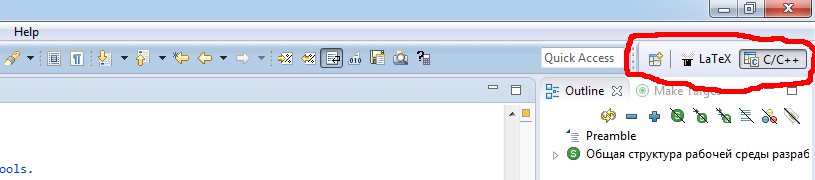
\includegraphics[width=0.9\textwidth]{fig/eclperpective.png}

\bigskip Для настройки привычных вам клавиш можно сразу зайти в
глобальные настроки среды и поменять привязку клавиш:

\bigskip\menu{Window>Preferences>General>Keys}

\menu{Type filter here:>F12}

\menu{Command}

\menu{Activate Editor>Binding>/удалить/}

\menu{Build Project>Binding>/нажать \keys{F12}/}

\menu{Apply>OK}




\secdown
\secru{Фичи}

Например нажатием \keys{F3}\ в \eclipse\ можно переместится на
  определение функции, на имени которой находится текствый курсор.
  
    Автодополнение\ --- редактор предлагает варианты полного написания
  идентификаторов и ключевых слов по первым буквам и нажатию обычно
  \keys{Ctrl+Tab} или \keys{Ctrl+N}. Также автоматически расставляются
  закрывающие скобки, закрывающие операторы управляющих структур типа begin/end,
  и генерируются синтаксические элементы циклов при вводе ключевых слов
  if/for/while. Особенно удобно автодополнение при написании кода на ООП 
  языках\  --- при вводе имени класса или объекта и точки предлагается меню с
  именами данных и методов класса. 
  
  При вводе имени функции и скобки выводится всплывающее окно с подсказкой\ ---
  определение функции с типом возвращаемого значения, типом и именами
  параметров.
  
  Интерфейс IDE часто предусматривает различные вспомогательные окна,
  показывающие имена и свойства объектов, описанных в программе (переменные,
  функции, структуры,..), структуру проекта с зависимостями между файлами, блоки
  справки в зависимости от текущего выделенного элемента и т.п.
  
  Часто IDE имеет встроенный графический интерфейс для отладки программ,
  используя для этого интерфейсные библиотеки для программатора и
  специальный отладочный код, добавляемый к вашей программе при
  компиляции. Используя аппаратный модуль отладки на целевом процессоре и
  отладочный код, IDE обеспечивает отображение значений и изменений регистров
  процессора, состояние переферии, позволяет задать точки останова в программном
  коде, в т.ч. условные по значению или измениею переменных или регистров
  железа.
  При использовании ОС реального времени и системы аппаратной многозадачности
  отображается загрузка ядер, загрузка процессора и используемые ресурсы для
  каждой задачи, работа планировщика, и т.п.
  
Для удобной работы доступно несколько бесплатных вариантов IDE, далее
рассмотрим два варианта: тяжелая суперуниверсальная среда \eclipse, и легкая 
в отношении требуемых ресурсов системы CodeLite.
  
\secup
	


\secru{САПР EDA KiCAD}

\cp{http://ru.wikibooks.org/wiki/KiCad}

KiCad\ --- распространяемый по лицензии GNU GPL программный комплекс класса EDA
с открытыми исходными текстами, предназначенный для разработки электрических схем и печатных плат.

Кроссплатформенность компонентов KiCad обеспечивается использованием 
библиотеки wxWidgets. Поддерживаются операционные системы Linux, 
Windows NT 5.x, FreeBSD и Solaris.

Разработчик\ --- Жан-Пьер Шарра (фр. Jean-Pierre Charras), исследователь 
в LIS (фр. Laboratoire des Images et des Signaux — Лаборатория Изображений 
и Сигналов) и преподаватель электроники и обработки изображений в фр. 
IUT de Saint Martin d’Hères (Франция).

\bigskip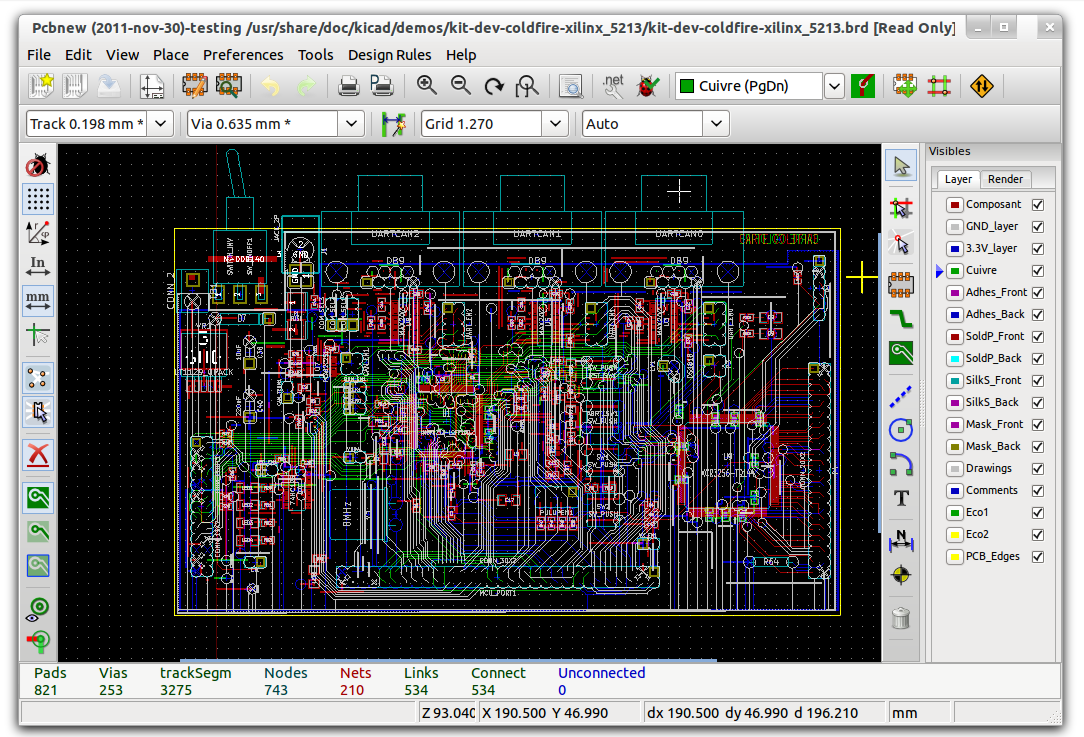
\includegraphics[height=0.5\textheight]{kicad/kicad_pcbnew.png}



\labwork{Установка KiCAD}\label{kicadinstall}

\bigskip
\menu{\wcmd{\url{http://www.kicad-pcb.org/}}>Download>KiCAD for OS }

\bigskip\menu{\file{KiCad\_stable-2013.07.07-BZR4022\_Win\_full\_version.exe}}

\bigskip

\menu{Installer Language>Russian>Ok}

\menu{Установка KiCAD 2013.07.07>Далее}

\menu{Лицензия>Принимаю}

\menu{Компоненты>\checkbox\ все>Далее}

\menu{Папка установки>\file{C:/Program Files/KiCad}>Установить}

\menu{Копирование файлов}

\menu{Завершение установки>\checked\ Wings3D>Готово}

\bigskip

\wcmd{\url{http://www.wings3d.com/}}



\secdown
\secru{kicad\ --- менеджер проектов}


\secru{eeschema\ --- редактор электрических схем}

обеспечивает:

\begin{itemize}
\item создание однолистовых и иерархических схем,
\item проверку их корректности ERC (контроль электрических правил),
\item создание списка электрических цепей netlist для редактора топологии платы
pcbnew или для Spice-моделирования схемы, 
\item доступ к документации на используемые в схеме электронные компоненты
(datasheet).
\end{itemize}
\secru{pcbnew\ --- редактор печатных плат}

обеспечивает:

\begin{itemize}
\item разработку плат, содержащих до 16 слоёв меди и до 12 технических слоёв
  (шелкография, паяльная маска и т. п.), 
\item выход на внешние трассировщики соединений посредством генерации описания 
платы на Specctra Design Language (on-line FreeRoute и др.),
\item генерацию технологических файлов для изготовления печатных плат
(Gerber-файлы для фотоплоттеров, файлы сверловок и файлы размещения компонентов), 
\item послойная печать схем и чертежей печатных плат на принтере или плоттере (в
форматах PostScript, HPGL, SVG и DXF), с рамкой формата или без неё.
\end{itemize}

\secru{gerbview\ --- просмотрщик файлов Gerber (фотошаблонов)}

позволяет просматривать Gerber-файлы.


\secru{cvpcb\ --- программа для выбора посадочных мест, соответствующих компонентам
на схеме}
\secru{wyoeditor\ --- текстовый редактор для просмотра отчётов}
\secru{Библиотеки компонентов}

В составе KiCad поставляются библиотеки электронных компонентов 
(обычных и поверхностно монтируемых SMD). Для многих библиотечных 
компонентов есть 3D-модели, созданные в Wings3D.

Компоненты и посадочные места корпусов можно ассоциировать с документацией, 
ключевыми словами и осуществлять быстрый поиск компонента по 
функциональному назначению.


\secup


% % % \part{\cmsis}
% % % \section{\copyright}
\cp{двойной лось
\url{http://www.doulos.com/knowhow/arm/CMSIS/CMSIS\_Doulos\_Tutorial.pdf}}

\bigskip
This tutorial material is part of a series to be published progressively by
Doulos.

\ru{Этот учебный материал является частью регулярных публикаций ДвухЛосей}

\bigskip
You can find the full set of currently published Tutorials and register for
notification of future additional at \url{www.doulos.com/knowhow}

\ru{Вы можете найти полный набор опубликованных методичек и зарегестироваться
для получения оповещений о новых выпусках на \url{www.doulos.com/knowhow}.}

\bigskip
You can also download the full source code of the examples used within the
Tutorial at the same URL.

\ru{По тому же URLу вы также можете скачать полную версию исходных кодов
примеров.}

\bigskip
Also check out the Doulos ARM Training and service options at
\url{www.doulos.com/arm}

\ru{Также посмотрите варианты учебных курсов Duolos по ARMам на
\url{www.doulos.com/arm}.}

\bigskip
Or email \email{info@doulos.com} for further information

\ru{Или запросите дополнительную информацию по \email{info@doulos.com}}

\bigskip
First published by Doulos March 2009

\ru{Первая публикация от Duolos Март 2009}

\bigskip
Copyright 2009 Doulos. All rights reserved. All trademarks acknowledged. All
information is provided “as is” without warranty of any kind.

\section{Введение}

The Cortex Microcontroller Software Interface Standard (CMSIS) supports
developers and vendors in creating reusable software components for 
\arm\ \cm{}\ based systems.

\ru{
Cortex Microcontroller Software Interface Standard (CMSIS)\footnote{стандарт
программного интерфейса микроконтроллеров Cortex}\ обеспечивает разработчикам и
производителям МК создание повторно используемых программных компонентов для
систем на основе микроконтроллеров \cm{}.
}

The \arm\ \cm{3}\ processor is the first core from ARM specifically designed for
the Microcontroller market. This core includes many common features (NVIC,
Timer, Debug-hardware) needed for this market. This will enable developers to
port and reuse software (e.g. a real time kernel) with much less effort to
\cm{3}\ based MCUs.

\ru{
Процессор \arm\ \cm{3}\ первое ядро от компании \arm\ специально разработанное
для рынка микроконтроллеров. Это ядро включает множество типовых блоков (NVIC,
таймеры, отладочный интрефейс) необходимых на этом рынке. Это позволяет
разработчикам с минимальными усилиями портировать и повторно использовать уже
написанное ПО\footnote{например ядро ОС реального времени}\ для МК семейства
\cm{3}\ любых производителей.
}

With a significant amount of hardware components being identical, a large
portion of the Hardware Abstraction Layer (HAL) can be identical. However,
reality has shown that lacking a common standard we find a variety of HAL/driver
libraries for different devices, which, as far as the \cm{3}\ part is
concerned essentially do the same thing\ --– just differently.

\ru{
Благодаря идентичности большого колиства аппаратных компонентов, также
идентичным оказывается и Hardware Abstraction Layer (HAL)\footnote{программный
слой аппаратной абстракции}.
Тем не менее, реальность показывает что отсутствие общего стандарта приводит к
множеству несовместимых версий библотек HAL и драйверов для различных МК, что не
соответствует идее полной переносимости ПО в серии \cm{3}.
}

The latest study of the development for the embedded market shows that software
complexity and cost will increase over time, see figure left.
Reusing Software and having a common standard to govern how to write and debug
the software will be essential to minimising costs for future developments.

\ru{
Последние исследования разработок для рынка встраиваемого ПО показывают, что
сложность программного обеспечения и его стоимость постоянно увеличиваются.
Повторное использование кода и наличие общего стандарта управляющего способами
написания и отладки ПО необходимы для минимизации стоимости разработки и
сопровождения.

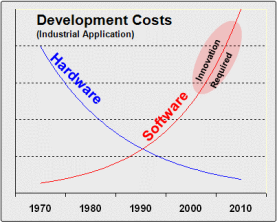
\includegraphics[height=30ex]{duolos_CMSIS/cmsisdevcosts.png}
стоимости разработки
}

\bigskip
With more \cm{3}\ based MCUs about to come onto the market, ARM has recognized
that after solving the diversity issue on the hardware side, there is still a
need to create a standard to access these hardware components.

\ru{
Анализируя ситуацию с взрывным ростом количества моделей МК \cm{3}\ на рынке,
компания \arm\ обнаружила что полная идентичность аппаратной части недостаточна
для обеспечения совместимости, и необходимо создание стандарта доступа к
аппаратным компонентам.
}

The result of that effort is CMSIS; a framework to be extended by vendors, while
taking advantage of a common API (Application Programming Interface) for core
specific components and conventions that define how the device specific portions
should be implemented to make developers feel right at home when they reuse code
or develop new code for ARM \cm{}\ based devices.

\ru{
Результатом этих исследований является \cmsis: фреймворк, расширямый
поставщиками МК, с сохранением полезных свойств общего API (Application
Programming Interface)\footnote{прикладной программный интерфейс} для ядреных
компонентов и соглашениями о том, как должны быть реализованы части зависимые от
железа, чтобы разработчики чувствовали себя как дома при повторном использовании
ил разработки нового кода для семейства \cm{}.
}

\section{Структура \cmsis}

CMSIS can be divided into three basic function layers:

\ru{\cmsis\ может быть поделен на три основных слоя:}

\begin{itemize}
\item Core Peripheral Access Layer (CPAL)

The lowest level defines addresses, and access methods for common components and
functionality that exists in every Cortex-M system. Access to core registers,
NVIC, debug subsystem is provided by this layer. Tool specific access to special
purpose registers (e.g. CONTROL, xPSR), will be provided in the form of inline
functions or compiler intrinsics. This layer will be provided by ARM.

\ru{
Самый нижний уровень определяет адреса, и методы доступа к общим компонентам и
функциям, существующим в каждой \cm{}-системе. Этим уровнем
описывается доступ к регистрам ядра, NVIC\footnote{Nested Vector Interrupt
Controller, контроллер вложенных прерываний}, подсистеме отладки.
Инструментальный доступ к спецрегистрам (\file{CONTROL},\file{xPSR})
предоставляется в форме inline-функций или интринсик компилятора. Этот уровень
обеспечивается лицензиатом архитектуры\ --- компанией \arm.
}

\item Middleware Access Layer (MWAL)

This layer is also defined by ARM, but will be adapted by silicon vendors for
their respective devices.
The Middleware Access Layer defines a common API for accessing peripherals. The
Middleware Access Layer is still under development and no further information is
available at this point.

\ru{
Этот слой также специфицируется \arm, но адаптируется производителем кристаллов
для их конкретных изделий. Слой MWAL определяет общий API для доступа к
периферии. Этот слой все еще находится на стадии доработки, и на текущий момент
более подробная информация неступна.
}

\item Device Peripheral Access Layer (DPAL)

Hardware register addresses and other definitions, as well as device specific
access functions will be defined in this layer. The Device Peripheral Access
Layer is very similar to the Core Peripheral Access Layer and will be provided
by the silicon vendor. Access methods provided by CPAL may be referenced and the
vector table will be adapted to include device specific exception handler
address.

\ru{
Слой содержит адреса аппаратных регистров и другие определения, в том числе
функции доступа к специфичным особенностям чипов.
DPAL сильно похож на CPAL, но предоставляется поставщиком кристаллов.
В CPAL могут быть описаны методы доступа и адаптированная таблица векторов,
содержащая обработчики исключений, специфичные для конкретного МК.
}

While DPAL is intended to be extended by the silicon vendor, let’s not forget
about Cortex-M based FPGA products, which effectively put developers into the
position of a silicon vendor.

\ru{
DPAL предназначен для расширения вендором, но не стоит забывать о
FPGA-продуктах с примением \cm{}-ядер, которые ставят разработчиков в положение
вендора.
}

\end{itemize}

The basic structure and the functional flow is illustrated in the Figure 2. below.

\bigskip
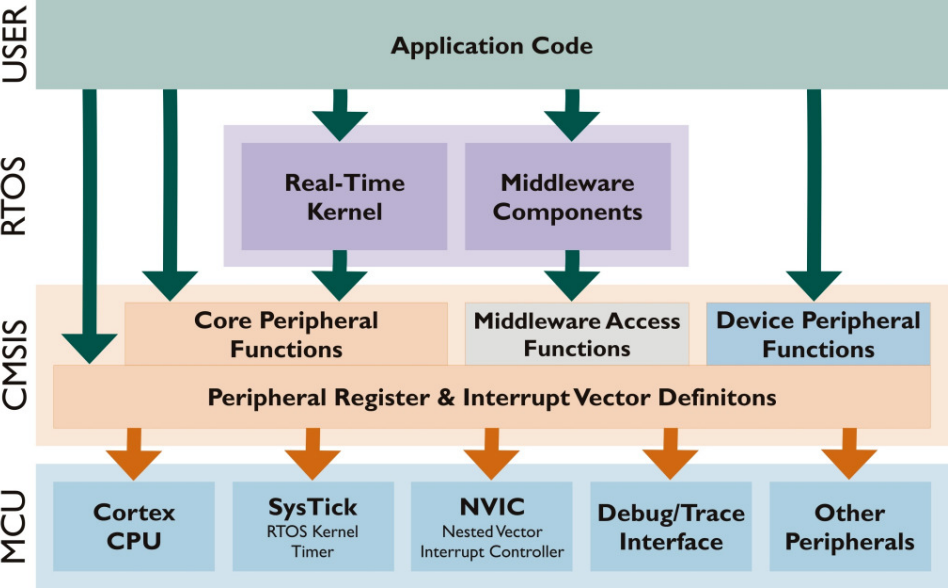
\includegraphics[width=0.9\textwidth]{duolos_CMSIS/cmsisstruc.png}

Figure 2 CMSIS Structure functional flow

\ru{Рис.2 Функциональная структура CMSIS}

\bigskip
As far as MCU based systems are concerned it might make sense for developers to
treat the entire PCB system as monolithic block. There is no reason to
differentiate between a memory mapped register inside the MCU and a memory
mapped register external to the MCU, connected via external memory interface.
The benefit of applying a standard like CMSIS is that existing guidelines on how
to access these devices set a clear goal on how to implement and integrate
critical parts of the software.
Other team members will find a familiar environment.

\subsection{Структура файлов}

File names in CMSIS are standardized as follows:

\begin{tcolorbox}
\begin{tabular}{l l}
\file{core\_cm3.h} &\cm{3}\ global declarations and definitions, static
function definitions \\
\file{core\_cm3.c} &\cm{3}\ global definitions\\
\file{<device>.h} &Top-level header file (device specific). To be included by
application code.\\
&Includes \file{core\_cm3.h} and \file{system\_<device>.h}\\
\file{system\_<device>.h} &Device specific declarations\\
\file{system\_<device>.c} &Device specific definitions, e.g.
\verb|SystemInit()|\\
\end{tabular}
\end{tcolorbox}

Application code will only include the top-level header file which implicitly
pulls in all other essential

\bigskip
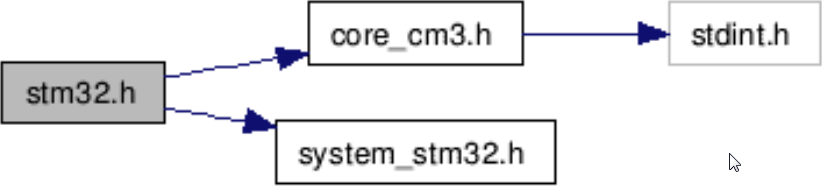
\includegraphics[width=0.5\textwidth]{duolos_CMSIS/stm32.png}
\bigskip

header files. The illustration below shows the flow and dependencies of the
header files \file{stm32.h}, \file{core\_cm3.h} and \file{system\_stm32.h},
which are part of CMSIS release V1P0.

\begin{lstlisting}[style=cpp]
/* Configuration of the Cortex-M3 Processor and Core Peripherals */
#define __MPU_PRESENT 0			 /*!< STM32 does not provide a MPU present or not*/
#define __NVIC_PRIO_BITS 4		 /*!< STM32 uses 4 Bits for the Priority Levels */
#define __Vendor_SysTickConfig 0 /*!< Set to 1 if different SysTick Config isused */
 
#include "core_cm3.h" 	 		 /* Cortex-M3 processor and core peripherals */ 
#include "system_stm32.h" 		 /* STM32 System */
\end{lstlisting}

The \file{<device>.h} file is the central include file and provided by the
silicon vendor. The application programmer is using that as the main include file in his
C source code. Note that the ARM \cm{3}\ has some optional hardware features
(e.g. the MPU, number of Interrupts and the number of the NVIC priority bits)
the silicon vendors may have implemented differently. The listing above shows
that STM32 implements four out of eight possible priority bits. The macro
\verb"__NVIC_PRIO_BITS"\ is set here to 4. STM32 does not offer a Memory
Protection Unit (MPU). Accordingly, the macro \verb"__MPU_PRESENT"\ has the
value 0.

The next example shows the corresponding definitions for a NXP LPC17xx device.
In this Cortex-M3 implementation five priority bits have been implemented and an
MPU is available.

\begin{lstlisting}[style=cpp]
/* Configuration of the Cortex-M3 Processor and Core Peripherals */
#define __MPU_PRESENT 1 		 /*!< MPU present or not */
#define __NVIC_PRIO_BITS 5 		 /*!< Number of Bits used for Priority Levels */
#define __Vendor_SysTickConfig 0 /*!< Set to 1 if different SysTick Config is used */

#include "..\core_cm3.h" 	/* Cortex-M3 processor and core peripherals */
#include "system_LPC17xx.h" /* System Header */
\end{lstlisting}

The \verb"__Vendor_SysTickConfig"\ defined is showing in both cases the default
setting. When this macro is set to 1, the \verb|SysTickConfig()|\ function in
the \file{cm3\_core.h}\ is excluded. In this case the file 
\file{<device>.h}\ must contain a vendor specific implementation of this
function.

\subsection{Независимость от тулчейна}

CMSIS exists in a three-dimensional space of the form
vendor$\div$device$\div$tool chain.
In order to remove one dimension (tool chain), the common files
\file{core\_cm3.c}\ and \file{core\_cm3.h}\ contain all essential tool specific
declarations and definitions.

\bigskip
Example:

\begin{lstlisting}[style=cpp]
/* define compiler specific symbols */
#if defined ( __CC_ARM )
	#define __ASM __asm				/*!< asm keyword for armcc */
	#define __INLINE __inline		/*!< inline keyword for armcc */
#elif defined ( __ICCARM__ )
	#define __ASM __asm				/*!< asm keyword for iarcc */
	#define __INLINE inline			/*!< inline keyword for iarcc.
									Only avaiable in High optimization mode! */
	#define __nop __no_operation	/*!< no operation intrinsic in iarcc */
#elif defined ( __GNUC__ )
	#define __ASM asm 				/*!< asm keyword for gcc */
	#define __INLINE inline 		/*!< inline keyword for gcc */
#endif
\end{lstlisting}

The remaining parts of CMSIS can now simply use the macro \verb|__INLINE|\ to
define an inline function.

\ru{Остальная часть \cmsis\ теперь может просто использовать макрос}
\verb|__INLINE|\ \ru{для определения инлайн-функций.}

\bigskip
Currently three of the most important C-compilers are supported: ARM RealView
(armcc), IAR EWARM (iccarm), and GNU Compiler Collection (gcc). This is expected
to cover the majority of tool chains.

\ru{
На настоящий момент поддерживаются три наиболее применяемых Си-компилятора:
ARM RealView (armcc), IAR EWARM (iccarm), и GNU Compiler Collection (gcc).
}

\subsection{Стандарт безопасности ПО MISRA-C}

Besides defining an API for Cortex-M core peripherals and guidelines on how to
support device peripherals, CMSIS defines some coding guidelines and
conventions. Most important is that the CMSIS code base is MISRA-C 2004
compliant, which implies that every extension should be compliant, too. MISRA-C
is a set of safety rules established by the “Motor Industry Software Reliability
Association” for the C programming language. Maintaining MISRA compliance can be
tricky, in particular when implementing driver level software. Therefore,
pragma-like exceptions in PCLint style are scattered across the source code. Be
aware that other tools, e.g. MISRA checker in IAR EWARM, might flag errors. Each
exception is accompanied with a comment explaining why this exception was made.

\subsection{Функции CPAL}

All functions in the Core Peripheral Access Layer are reentrant and can be
called from different interrupt service routines (ISR). CPAL functions are also
non-blocking\footnote{Memory barriers are exempt from that rule although they
might stall the processor for a few cycles.}\ in the sense that they do not 
contain any wait-loops.

The majority of functions in the CPAL have been implemented in the header file
\file{core\_cm3.h}\ as \verb|static| \verb|inline| functions. This allows the
compiler to optimize the function calls by placing the instructions that make up the called
function along with other code from which the function was called.

\subsection{Подпрограммы обработки прерываний}

Exception handlers will get a name suffix \verb|_Handler|, while (external)
interrupt handlers get the suffix \verb|_IRQHandler|. There must be a default
handler for each interrupt, which executes an infinite loop.
Tool specific configuration must make sure that this default handler will be
used as fall-back if no user-provided handler exists. It done
Through \verb|__weak| declaration in EWARM and RVCT armcc,
\verb|__attribute__((weak))| in GCC and RVCT armcc and
\verb|[WEAK]| export in RVCT/armasm.

Given that the \cm{}\ NVIC provides byte-arrays and bit-strings to configure
priorities and interrupt source en-/disable, an enumerated type \verb|IRQn_t|
with an element for each exception/interrupt position with the suffix
\verb|_IRQn|\ must be defined for each interrupt (\file{<device>.h}). The system
handler names are common for all devices and must not be changed.

\begin{lstlisting}[style=cpp,title=Listing shows the generic part of the
(\file{<device>.h}) file.] typedef enum IRQn
{
/****** Cortex-M3 Processor Exceptions Numbers *******************************/
 NonMaskableInt_IRQn = -14, 	/*!< 2 Non Maskable Interrupt */
 MemoryManagement_IRQn = -12, 	/*!< 4 Cortex-M3 Memory Mgmt Interrupt */
 BusFault_IRQn = -11, 			/*!< 5 Cortex-M3 Bus Fault Interrupt */
 UsageFault_IRQn = -10, 		/*!< 6 Cortex-M3 Usage Fault Interrupt */
 SVCall_IRQn = -5, 				/*!< 11 Cortex-M3 SV Call Interrupt */
 DebugMonitor_IRQn = -4, 		/*!< 12 Cortex-M3 Debug Monitor Interrupt */
 PendSV_IRQn = -2, 				/*!< 14 Cortex-M3 Pend SV Interrupt */
 SysTick_IRQn = -1, 			/*!< 15 Cortex-M3 System Tick Interrupt */
/****** Device specific Interrupt Numbers ************************************/
 UART_IRQn = 0, 				/*!< Example Interrupt */
} IRQn_Type;
\end{lstlisting}

All system handlers have negative virtual slot numbers so that they can be
distinguished in functions that abstract from the differences between system
handlers and external interrupt handlers. External interrupt handlers start at
the index 0.

\subsection{Другие соглашения о коде}

The CMSIS documentation recommends a few more things regarding capitalization of
identifiers, commenting code.

\subsubsection{Идентификаторы}

\begin{itemize}
  \item Capital names to identify Core Registers, Peripheral Registers, and CPU
  Instructions.
  
  E.g.: \verb|NVIC->AIRCR|, \verb|GPIOB|, \verb|LDMIAEQ|
  
  \item “CamelCase” (mix of upper- and lower-case letters) names to identify
  peripherals access functions and interrupts.

 E.g.: \verb|SysTickConfig()|, \verb|DebugMonitor_IRQn|

  \item Peripheral prefix (\verb|<name>_|) to identify functions that belong to
  specific peripherals.

 E.g.: \verb|ITM_SendChar()|, \verb|NVIC_SystemReset()|

\end{itemize}

\subsubsection{Комментарии}

CMSIS uses \term{Doxygen}\ style comments for all definitions and encourages
developers to do the same.

In particular, the comment for each function definition should at least contain

\begin{itemize}
\item one-line brief function overview. (Tag: \verb|@brief|)
\item detailed parameter explanation. (Tag: \verb|@param|)
\item detailed information about return values. (Tag: \verb|@return|)
\item detailed description of the actual function.
\end{itemize}

The example below shows the beginning of a function definition:

\begin{lstlisting}[style=cpp]
/**
 * @brief Enable Interrupt in NVIC Interrupt Controller
 *
 * @param IRQn_Type IRQn specifies the interrupt number
 * @return none
 *
 * Enable a device specific interupt in the NVIC interrupt controller.
 * The interrupt number cannot be a negative value.
 */
static __INLINE void NVIC_EnableIRQ(IRQn_Type IRQn)
{
// . . .
}
\end{lstlisting}

The tags can be parsed by the documentation tool Doxygen, which is used to
create cross-referenced source code documentation in various formats
(\url{http://www.stack.nl/~dimitri/doxygen/index.html}). The tag syntax is
rather minimalistic and does not impair readability of the source code. Please
consult the Doxygen Documentation for details about tag syntax.

As an alternative to regular C block comments (\verb|/* */|) CMSIS explicitly
allows line comments (\verb|//|, so called C++-comments). If you are concerned
about MISRA compliance, be aware though, that MISRA-C 2004 doesn’t allow line
comments according to rule 2.2.

\ru{
CMSIS предлагает альтернативу обычным сишным /* блочным комментариям */ в виде
// строчных комментариев, так называмых \cpp-комментариев. Если вас беспокоит
выполнение превил MISRA, учтите что} \alarm{MISRA-C:2004 не разрешает
использовать строчные комментарии согласно правилу 2.2}.

\subsubsection{Типы данных}

All data types referenced by CMSIS are based on those defined in the standard C
header file \file{stdint.h}. Data structures for core registers are defined
CMSIS header file \file{core\_cm3.h}, along with macros for qualifying registers
according to their access permissions. The rationale is that tools might be able
to automatically extract that information for debug purposes.

\begin{lstlisting}[style=cpp]
#define 	__I 	volatile const	/*!< defines 'read only' permissions */
#define		__O 	volatile 		/*!< defines 'write only' permissions */
#define 	__IO 	volatile 		/*!< defines 'read / write' permissions */
\end{lstlisting}

\subsection{Отладка}

A common requirement in software development is some sort of terminal output for
debugging. Text/graphics displays in embedded devices cannot be assumed to be at
hand (or might be in use), which previously left the developer with essentially 
two choices:

\begin{enumerate}
\item Use one of the ubiquitous UARTs and connect a terminal

Issues: All UARTs might be in use, access to UART signals might not be possible
for reasons that include pin-sharing, PCB layout, etc.

\item Use the semihosting mechanism

Issue: Significant software overhead on target CPU, might not be supported in
the same way by all tool chains, potential impact on timing behavior.
\end{enumerate}

With \cm{3}\ the preferred method makes use of the Instrumentation Trace
Macrocell (ITM), which is part of the processor macro cell and thus always
present.\footnote{Always present in \cm{3}\ rev1 cores. \cm{3}\ rev2 makes
ITM an optional feature.}

A Serial Wire Viewer (SWV) capable debug adapter can receive ITM data through
the SWO (Serial Wire Out) debug pin. ITM implements 32 general purpose data
channels. CMSIS builds on top of this and declares channel 0 to be used for
terminal output, along with a function called \verb|ITM_SendChar()| which can be
used as low-level driver function for printf-style output. A second channel (31) 
has been reserved for OS aware debugging, which means that a kernel can use it
to transmit kernel specific data which could then be interpreted by the debug
tool. 

With this standardization, tool vendors have it much easier to implement
specific debug features, such as e.g. terminal emulation for data received via
ITM channel 0. Developers on the other hand can rely on this feature to dump
state information, without having to configure UARTs and external terminal
emulators. See our Tutorial 2 later in this document.

Access privilege can be configured for groups of ITM channels. In order to use
ITM channel 0, unprivileged access must be granted, whereas ITM channel 31 is in
a different group and may allow privileged access only.

\subsection{Контроль версии CMSIS}

The CMSIS developers have taken care to provide macros indicating the CMSIS
version used in a project. That way provisions can be made to prevent code to be
used with a different CMSIS version than originally intended.

\ru{
Разработчики \cmsis\ позаботились о предоставлении макросов версии \cmsis,
использованной в проекте. Это способ для защиты от использования кода,
предназначенного для другой версии \cmsis.
}

\begin{lstlisting}[style=cpp]
#define __CM3_CMSIS_VERSION_MAIN (0x01)		/* [31:16] main version */
#define __CM3_CMSIS_VERSION_SUB (0x10)		/* [15:0] sub version */

#define __CM3_CMSIS_VERSION ((__CM3_CMSIS_VERSION_MAIN << 16) | \
							__CM3_CMSIS_VERSION_SUB)
\end{lstlisting}

\section{Урок 1 – Первый пример}

In order to explain application of CMSIS in real projects, we are going to look
at a simple example of a \cm{3}\ application. The program compiles for STM32
processors and a project file for the Keil $\mu$Vision IDE has been provided.
Porting the example to other tool chains, such as IAR EWARM is straight forward
and the IAR EWARM version is provided as well. A great number of CMSIS function
definitions can be found in \file{core\_cm3.h}\ as “static inline” functions.
Depending on the compiler optimization level, this helps getting very efficient
instruction sequences rather than actual function calls, while ensuring a
certain level of type safety.

After clock and GPIO initialization, the SysTick timer is configured to a period
of 0.5 seconds. Whenever the handler executes it toggles the state of
\verb|GPIOB[15]|.

\subsection{Пример 1 Точка входа}

Initially, the program was implemented using STMicroelectronics’ FWLib, a
library that provides access to \cm{3}\ internals and STM32 peripherals. Near
to medium term, firmware libraries such as FWLib will be based on CMSIS. Parts
of FWLib that will eventually form the DPAL (see above).

\lstinputlisting[inputencoding=cp1251,style=cpp]{duolos_CMSIS/stm1.c}

\lstinputlisting[inputencoding=cp1251,style=cpp]{duolos_CMSIS/stm2.c}

The two listings above show the contents of main.c, and \file{stm32f10x\_it.c}.
This latter file contains interrupt handler templates from ST’s FWLib, which
have to be adapted to implement project specific functionality.

\subsection{Пример 2 Адаптация для CMSIS}

In a second step, the program has been converted to using CMSIS. The CMSIS
version used is V1P10 as downloaded via the link above. We want to make sure to
use the same CMSIS that has been used to develop the program and check the
version number.

\lstinputlisting[inputencoding=cp1251,style=cpp]{duolos_CMSIS/stm3.c}

Initial support for STM32 MCU is part of CMSIS and is pulled in by including the
header file \file{stm32.h}. At the point of writing this tutorial a fully CMSIS
complaint FWLib was not available so some compromises and hand adjustments hand
to be made. Fore this reason, we will include both, FWLib and CMSIS files. Until
vendors have full adopted CMSIS small issues will have to be dealt with when
combining CMSIS with a vendor library.

In this case simply including the FWLib main header file \file{stm32f10x\_lib.h}
in addition to \file{stm32.h} triggers a number of error messages caused by
multiple definitions of functions and macros. To avoid this, we will have to
selectively include individual FWLib headers (see below). All FWLib headers
depend on definitions in the files \file{cortexm3\_core.h} and
\file{stm32f10x\_map.h}. Most of the definitions in these two header files have
already been defined by CMSIS (\file{core\_cm3.h} and \file{system\_stm32.h})
and we have to pretend to FWLib that both header files had been included already.

\begin{lstlisting}[style=cpp]
// Prevent interference with FWLib
#define __STM32F10x_MAP_H
#include <stm32f10x_type.h>
#include <stm32f10x_gpio.h>
#include <stm32f10x_rcc.h>
\end{lstlisting}

Actual system initialization will be encapsulated by the CMSIS function
\verb|SystemInit()|, which has to be implemented by the silicon vendor. As a
minimal requirement, this function would initialize the MCU’s clock system. In
case of the reference implementation in \file{system\_stm32.c},
\verb|SystemInit()| also initializes the Flash memory interface. CMSIS defines a
single system variable, \verb|SystemFrequency|, which is supposed to reflect the
frequency of both core and SysTick timer in Hz. This concept is sufficient for a
minimal implementation but will likely have to be extended for actual MCU as
demonstrated by CMSIS’ \file{system\_stm32.c}, in which several variables have
been defined to hold the frequency values of different clock domains in the
STM32 MCU. SysTick timer and core could have different frequencies and care must
be taken when using SystemFrequency in a program.

Current CMSIS does not initialize peripheral clocks and it is arguable whether
it should. In any case we use the corresponding FWLib function to enable GPIOB
clock.

\begin{lstlisting}[style=cpp]
// Initialization moved to SystemInit() in system_stm32.c. Clock
// configuration now handled by #defines. Use uVision
// configuration wizard or text editor to change.
SystemInit(); 										// *** CMSIS change ***
// APB peripherals still have to be enabled individually.
RCC_APB2PeriphClockCmd(RCC_APB2Periph_GPIOB, ENABLE);
\end{lstlisting}

NVIC group- and sub-priority configuration is handled by the function
\verb|NVIC_SetPriorityGrouping()|, where the direct encoding of the
\verb|PRIGROUP| field in \verb|SCB->AIRCR| is used. We choose the value 4, which
represents 3 bits for group (preempting) and 5 bits for the sub priority. A
general formula to calculate the proper value is \verb|PRIGROUP = bitssub-1|.

\begin{lstlisting}[style=cpp]
// priority configuration: 3.5
NVIC_SetPriorityGrouping(4); 		// *** CMSIS change ***
\end{lstlisting}

Different from the initial version of the example, the CMSIS variant does not at
this point set the SysTick handler priority. This is part of the SysTick
initialization and will be covered later.

\begin{lstlisting}[style=cpp]
GPIO_Init(GPIOB, &GPIOB_InitStruct);
GPIO_WriteBit(GPIOB, GPIO_Pin_All, Bit_RESET);
\end{lstlisting}

Following NVIC set-up, we use plain FWLib functions to configure GPIO port B.

\begin{lstlisting}[style=cpp]
SysTick_Config(SystemFrequency/2); // *** CMSIS Change ***

// SysTick_Config() hardcodes priority. We will overwrite this.
NVIC_SetPriority(SysTick_IRQn, 14); // *** CMSIS change ***
\end{lstlisting}

\verb|SysTick_Config()|, provided by CMSIS, programs the reload register with
the parameter value. The function also selects HCLK (core clock) as clock
source, enables SysTick interrupts and starts the counter. The function also
fixes the SysTick handler priority to the lowest priority in the system, which
is the recommended SysTick priority for use in an RTOS scheduler for instance.
In our example, however, we prefer a different priority and override the hard
coded value with an additional call to \verb|NVIC_SetPriority()|. This function
abstracts from the difference between \cm{3}\ system handlers and external
interrupt handlers. All configurable system exceptions will be identified by
negative IRQ numbers (see above).

\begin{lstlisting}[style=cpp]
__irq void SysTick_Handler()
{
	static BitAction toggle = Bit_SET;
	GPIO_WriteBit(GPIOB, GPIO_Pin_15, toggle);
	if (toggle == Bit_SET) {
		puts("Pin state is ON");
		toggle = Bit_RESET;
	} else {
		puts("Pin state is OFF");
		toggle = Bit_SET;
	}
}
\end{lstlisting}

The SysTick handler code above does not need any modification. FWLib naming
conventions is complying with CMSIS, in that the names of all internal exception
handlers must end in \verb|_Handler|. Names of external interrupt handlers must
end in \verb|_IRQHandler|. The handler implementation accesses the GPIO port via
FWLib functions and definitions.

\section{Урок 2 – ITM Отладка}

To exercise some CMSIS debug functionality for our first example from tutorial
1, we add debug output messages via calls to \verb|puts()|. We will now redirect
character output to Instrumentation Trace Macrocell (ITM), (remember that CMSIS
reserves ITM channel 0 for this), using the CMSIS function
\verb|ITM_SendChar()|. A mechanism called retargeting enables us to provide our
own implementation of a system function.

\begin{lstlisting}[style=cpp]
// retarget fputc() for debug output via ITM
int fputc(int c, FILE *stream) {
	return (int)ITM_SendChar((uint32_t)c);
}
\end{lstlisting}

The standard C function \verb|fputc()|, which will eventually be called by
\verb|puts()| in our SysTick handler, will be re-implemented, taking advantage
of the function \verb|ITM_SendChar()|. The result of this retarget can now be
easily monitored in $\mu$Vision ITM viewer as shown in the screenshot below.

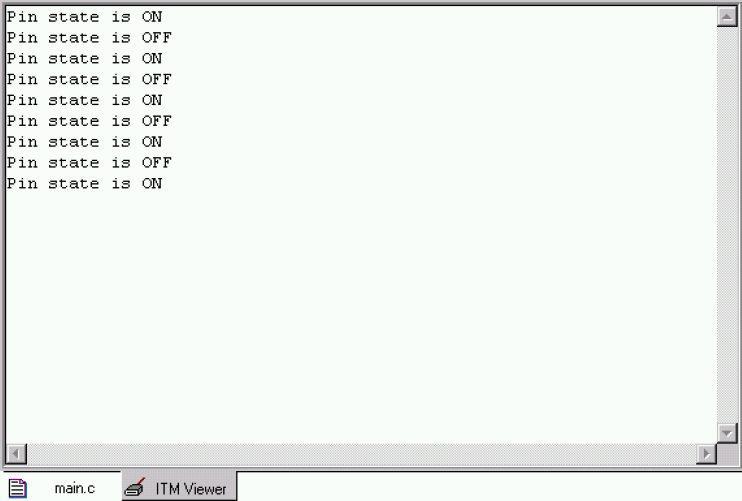
\includegraphics[width=0.5\textwidth]{duolos_CMSIS/ITMshot.png}

If you are going to use the IAR EWARM tool for this example it is not necessary
to manually retarget this function. Instead, in the project options dialog under
“General Options” there is a tab “Library Configuration” tab, which offers
checkboxes to enable this functionality. The screenshot below shows which
settings are required to redirect standard output.

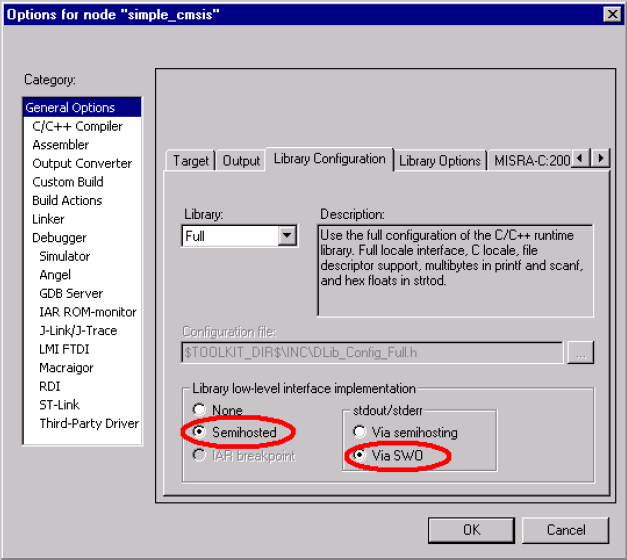
\includegraphics[width=0.6\textwidth]{duolos_CMSIS/simplecmsis.png}

\section{Заключение}

The CMSIS will reduce the learning-curve for the application programmers by
providing a consistent software framework, ensuring consistent documentation and
easy deployment of boilerplate code across various compiler vendors. The
consequent use and implementation of CMSIS across many silicon and middleware
software partners will simplify the verification and certification process and
therefore reduce future project risk. The adapted common programming techniques
though CMSIS will simplify the long term maintenance due to easier to understand
source code. The silicon vendors can focus on there added value and device
features. All reasons together will reduce software development cost and time to
get new products to the market.

% 
% % \chapter{Первые шаги}
% % \labpart{Первые шаги}
% % \labwork{Создание нового проекта в \eclipse}\label{labecreprj}

Создадим новый проект, напишем простую программу, и запустим ее в отладчике.

\bigskip\menu{\eclipse>File>New>Project>C/C++>C Project>Next}

\menu{Project name>hello}

\menu{Project type>Makefile project>Empty project}

\menu{Toolchains>Cross ARM GCC}

\menu{Finish}

\menu{This kind of project associated with C/C++ perspective>Yes}

% % \labwork{Создание Makefile}\label{labmkmake}

Стоит объяснить, почему при создании проекта мы выбрали тип \file{Makefile
project}, хотя были доступны более логичные варианты типа \file{ARM C Project}.

Утилита \make\ ведет свою историю с 70х гг. Компьютеры тогда были большими,
тяжелыми, а главное медленными и с очень маленькой памятью (десятки$\div$сотни
Кб).
Компиляторам зачастую не хватало памяти, чтобы скомпилировать большую программу.
Кроме того, скорость их запуска и работы была тоже черепашьей.
Поэтому исходный код программы делили на модули, компилировали или
ассемблировали каждый модуль по-отдельности в \term{объектный код}, а затем уже
на конечном этапе с помощью \term{линкера}\ собирали несколько файлов объектного
кода в один исполнямый файл.

Для ускорения и упрощения этого процесса и была создана утилита \make.
Чтобы не вызывать лишний раз компилятор или какой-нибудь транслятор, в файле
\makefile\ прописываются зависимости между файлами. Затем запускается \make\ c
указанием какой файл нам нужно получить, и выполняется цепочка вызовов
нужных программ.

Следует отметить, что утилита \make\ используется до сих пор для сборки самых
современных программных пакетов (типа GCC 4.9.x), правда в комплексе с другими
средствами, обеспечивающими переносимость программ между разными ОС и
автогенерацией зависимостей из исходного кода.

\bigskip
Для наших целей \make\ используется как самое простое средство управления
компиляцией проекта. В средах разработки, особенно в коммерческих,
используются служебные файлы проектов, иногда бинарные, чаще текстовые, но
всегда запутанные и весьма развесистые.

Если вам вдруг понадобится откомпилировать ваш проект на другом компьютере,
с другой архитектурой, возможно вообще без графического
интерфейса\footnote{например какой-нибудь удаленный сервер на
процессоре 1995ВМ666 под раскряченным Solaris 7$\alpha$4, на котором лежит
криптобиблиотека, использующая при компиляции трофейный электро-механический 
энкодер, существующий в единственном экземпляре \smiley}, или вы вдруг решите
попробовать работать в другой IDE\ --- вы тут же вляпаетесь в ситуацию, 
когда нечем открыть файл проекта с заботливо прописанными опциями
компиляции.

\bigskip
\menu{\eclipse>\window{Project Explorer}>\file{hello}>\rms>Open Project}

\menu{\eclipse>\window{Project Explorer}>\file{hello}>\rms>New>File>File
name:>\file{Makefile}}

\bigskip
\lstinputlisting[style=mk,inputencoding=cp1251]{tmp/hello.mk}

\bigskip
Этот пример \makefile\ достаточно универсален и самодостаточен для большинства
проектов в этой книге. Кажущийся большой объем получился за счет использования
комментариев и переменных. И те, и другие служат для документирования проекта,
и повышают читаемость кода. В принципе никто не мешает\footnote{особенно для
микроскопических объемов исходных текстов программ для контроллеров\ ---
в самом худшем случае какие-то жалкие сотни Кб}\ написать несколько строк в
\file{.bat}нике с явным указанием опций компиляторам, или вообще откомпилировать
все исходники сразу одним вызовом \file{gcc}\ с кучей опций и списком исходных
файлов. Но если вам потребуется что-то изменить, куда проще и быстрее сделать
это в аккуратно оформленном самодокументированном \makefile.


% % 
\labwork{Hello World}\label{labhello}

Для начала нужно рассмотреть набор файлов минимального проекта:

\begin{itemize}

\item \file{README.txt}

Краткая информация о проекте\ --- название, авторы, обязательно ссылки на
\git-репозиторий, сайт, форум, и т.п.
 
\item \file{Makefile}

Файл с описанием зависимостей между файлами, настройками проекта (в переменных)
и правилами вызова компиляторов.

\item \file{startup.S}

Стартовый код процессора, включает инициализацию системы тактирования, мапинга
памяти, контроллера прерываний и минимальную инциализацию периферии.
Пишется на ассемблере, т.к. на Си получается слишком сложно, синтаксически
запутанно, или очень специфично для компилятора.

\item \file{startup.c}

Сишный вариант стартового кода, использование синтаксических ухищрений
GNU CC позволяет обойтись без ассемблера даже для описания таблицы векторов,
но для начинающего сложновато разобраться.

\item \file{init.c}

Сишный код инициализации железа (синтаксически легче описать блоки кода,
зависимые от целевого процессора).

\item \file{main.c}

Основной код, решающий поставленную задачу. 

\item \file{\$CPU.ld}

Скрипт линкера, настраивающий генерацию выходного бинарного файла в 
зависимости от целевого процессора\ --- прежде всего организация памяти,
и размещение сегментов кода/данных по фактическим адресам памяти.
Поэтому здесь имя файла задано через переменную, описанную в \makefile.

\item \file{generic.ld}

Скрипт линкера, содержащий общую часть для всех микроконтроллеров

\end{itemize}

\bigskip Создаем эти файлы аналогично \makefile\ в \labref{labmkmake}:

\bigskip\menu{\eclipse>\window{Project Explorer}>\file{hello}>\rms>New>File>File
name:>\file{НужныйФайл.xxx}}

\lstinputlisting[inputencoding=cp1251,title=README.txt]{hello/README.txt}

\lstinputlisting[style=asm,inputencoding=cp1251,title=startup.S]{hello/startup.S}

\lstinputlisting[style=cpp,inputencoding=cp1251,title=init.c]{hello/init.c}

\lstinputlisting[style=cpp,inputencoding=cp1251,title=main.c]{hello/main.c}

\lstinputlisting[style=gnuld,inputencoding=cp1251,title=arm7tdmi.ld]{hello/arm7tdmi.ld}

% % \labwork{Настройка отладчика в \eclipse}\label{labgdbinst}

\cp{http://makesystem.net/?p=2146}

 На сегодняшний день существуют много способов и инструментов для отладки
 embedded приложений, начиная с отладки “в железе” (внутрисхемная отладка)  и
 заканчивая всякими симуляторами. У каждого метода есть свои плюсы и минусы, но
 поскольку мы будим писать приложения для реальных устройств, то
 предпочтительней реальная отладка (в железе), то есть приложение будит
 исполняться непосредственно микроконтроллером.
 
Что нам понадобится для “железной отладки” :

\begin{itemize}
  \item 
ARM микроконтроллер (для симуляции необязателен)
  \item 
JTAG/SWD адаптер (для симуляции необязателен)
  \item 
GDB сервер (транслятор интерфейсов GDB/JTAG)
  \item 
GDB отладчик (имеет встроенный симулятор ARM7TDMI, используется для первых лаб) 
  \item 
плагин C/C++ GDB Hardware Debugging 
  \item 
плагин Eclipse Embedded Systems Register View 
\end{itemize}

\term{JTAG адаптер}\ (он же \term{программатор}) следует выбрать тот, который
поддерживает именно ваш микроконтроллер, а еще лучше, микроконтроллеры разных
производителей.
В моем случае (еще с давних времен у меня завалялись кристаллы от Texas
Instruments, ST Microelectronics, NXP, Atmel, Cypress), я сразу решил найти
программатор поддерживающий имеющиеся у меня камни. Порыскав в интернетах, мой
выбор пал на китайский клон знаменитого J-Link, в добавок к которому идет уйма
полезных утилит от Segger Microcontroller (тут обошлось без китая \smiley),
облегчающие жизнь разработчику.

В этой книге также рассмотрено несколько простых варинтов JTAG-адаптеров,
которые вы можете сделать сами, не обладая выдающимися знаниями в электронике
и технологиях производства печатных плат.

\bigskip
Структура аппаратно-программного комплекта для отладки:

\menu{микроконтроллер>JTAG/SWD>адаптер>LPT/USB>GDB сервер>протокол
GDB>GDB отладчик>IDE}

Адаптер подключается к выводам МК с помощью колодки (JTAG) или гребенки (SWD).

К компьютеру адаптер подключается через однин из распространенных интерфейсов:
совсем дешевые варинты ``на пяти резисторах'' через порт LPT, чуть подороже
через USB, совсем дорогие проф.модели могут иметь Ethernet интерфейс.

\bigskip
\term{Отладчик}\ (дебаггер, англ. debugger)\ --- компьютерная программа,
предназначенная для поиска ошибок в других программах. Отладчик позволяет
выполнять пошаговую трассировку, отслеживать, устанавливать или изменять
значения переменных в процессе выполнения кода, устанавливать и удалять
контрольные точки или условия остановки, сопоставлять двоичный код\ --- eгo
исходному тексту (на основе которых можно точно определить выполняемые
программой действия) и т.д. (Wiki)

Практически во все тулчейны входит утилита GDB (\file{arm-none-eabi-gdb}), это и
есть отладчик GNU. В принципе, дебаггер выполняет два типа действий:
управление исполнением программы в кристалле (через отладочный интерфейс) и
вывод результатов в консоль/графическую оболочку.

\bigskip
При сборке тулчайна (из исходников) невозможно заранее сказать, какой набор
отладочных средств будет у конечного пользователя\ --- у типичного
ембеддера\footnote{разработчика ПО под встраиваемые системы}\ запросто наберется
пара-тройка различных \jtag-адаптеровв, несколько демоплат со
встроенным адаптером, причем с разными процессорами, несколько собственных
устройств с самодельными отладочными интерфейсами, и еще для комплекта пару
чисто программных симуляторов \arm-ядер.

Задачу унификации интерфесов, и подключения всего этого зоопарка к одному и тому
же отладчику \gdb\ выполняет \term{\gdb-сервер}. Отладчик общается с сервером по
одному и тому же унифицированному \term{\gdb-протоколу}\ через последовательный
порт или TCP/IP соединение, а все сложности взаимодействия с железом берет на
себя сервер.
Это сделано (в том числе) для тех случаев, когда \gdb-отладчик работает на одном
ПК а \gdb-сервер на другом (в соседней комнате или соседнем государстве
\smiley). Опять же, сервер надо выбрать тот, который поддерживает ваш
\jtag-адапер или эмулятор.

\bigskip
\gdb, как и все остальные утилиты тулчайна, работает из командной строки, что
не всем удобно \smiley, поэтому для начала стоит научиться им пользоваться из
графической оболочки. \eclipse\ как и подобает серьёзной IDE, имеет средства
работы с \gdb, заменяющие его консоль, имеет графические кнопки для вызова
всех отладочных команд, и отображает содержимое регистров, памяти и т.п. в
графических окнах. Взаимодействие \eclipse/\gdb\ обеспечивает плагин \file{C/C++
GDB Hardware Debugging}, входящий в состав уже установленного ранее
расширения \file{CDT}.

\bigskip
Проверить наличие плагина можно так:

\menu{Help>Install New Software>Work with:>All Available Sites}

\menu{\uncheckbox\ Hide items that are already installes}

\menu{type filter>GDB}

\dirtree{%
.1 GDB.
.2 CDT Optional Features.
.3 \checkbox\ C/C++ GDB Hardware Debugging.
.2 Mobile and Device Development.
.3 \checkbox\ C/C++ GDB Hardware Debugging.
}

\bigskip

Прежде всего отключим оптимизацию кода проекта, задав в
\makefile\ значение переменной \file{OPTFLAGS = -O0}. 

Затем, нужно включить в проекте генерацию отладочной информации\footnote{имена
переменных, функций и т.п. объектов программы, в т.ч. и сами строки исходного
кода}, добавив опцию \file{-g[N]}.

Существуют три уровня отладочной информации:

\begin{enumerate}
\item в объектный код вставляется минимальный объем отладочной информации. Ее
вполне достаточно для трассировки вызовов функций и исследования глобальных
переменных, тем не менее, отсутствует информация для сопоставления выполняемого
кода со строками исходного кода и информация для отслеживания локальных
переменных.

\item используется по умолчанию. Помимо всей отладочной информации пepвoгo
уровня он дополнительно включает данные, необходимые для сопоставления строк
исходного кода с выполняемым кодом, а также имена и расположение локальных
переменных.

\item помимо всей отладочной информации пepвoгo и второго уровней, включает
дополнительную информацию, в частности определения макросов препроцессора.
\end{enumerate}

Используем 3 уровень, изменив в \makefile\ значение переменной 
\file{DEBFLAGS = -g3 -ggdb}. Опция \term{-ggdb}\ задает дополительно формат
отладочной информации. Доступны форматы STABS, DWARF2 и родной формат платформы.

В файле \file{startup.o.dump}\ при этом появляются дополнительные секции
с отладочной информацией, и в заголовок добавляются флаги, указывающие на
ее наличие:

%\lstinputlisting[style=objdump,title=startup.o.objdump]{hello/startup.o.objdump}
\begin{lstlisting}[style=objdump,title=startup.o.objdump]
startup.o:     file format elf32-littlearm
architecture: armv4t, flags 0x00000011: HAS_RELOC, HAS_SYMS
...
  4 .debug_line   00000044  00000000  00000000  000000b0  2**0
                  CONTENTS, RELOC, READONLY, DEBUGGING
  5 .debug_info   00000044  00000000  00000000  000000f4  2**0
                  CONTENTS, RELOC, READONLY, DEBUGGING
  6 .debug_abbrev 00000014  00000000  00000000  00000138  2**0
                  CONTENTS, READONLY, DEBUGGING
  7 .debug_aranges 00000020  00000000  00000000  00000150  2**3
                  CONTENTS, RELOC, READONLY, DEBUGGING
\end{lstlisting}   

\bigskip
Для настройки отладочного интерфейса заходим в меню

\menu{Run>Debug Configurations\ldots}

\menu{GDB Hardware Debugging>\rms>New}

В результате открывается окно с настройками отладки.

\bigskip
Для начала попробуем работу нашей прошивки на встроенном в \gdb\ программном
симуляторе процессора \file{ARM7TDMI}.

\bigskip
Вкладка Main.

\bigskip
В поле Name, можно дать имя всей конфигурации отладки, поскольку даже для одного
проекта бывают разные конфигурации отладки (скажем для отладки в RAM или Flash
памяти).

\menu{Name:>ARM7TDMI simulator}

В поле Project указываем имя проекта (поскольку в нашем workspace может быть
более одного проекта)

\menu{Project:>hello}

В поле C/C++ Application указываем имя *.elf файла сгенерированного после
компиляции (с введенными ранее настройками для Debug прошивки) проекта и который
будет использован во время отладки.

\menu{C/C++ Application:>startup.o}

\alarm{Перед тем как перейти к следующей вкладке, в нижней части окна
обязательно выбираем}

\menu{Legacy GDB Hardware Debugging Launcher}

\menu{Apply}

\bigskip
Вкладка Debugger. Здесь мы установим связь между отладчиком и графической
оболочкой, а также между отладчиком и \gdb-сервером (отсюда и название вкладки).

\bigskip
В поле GDB Command указываем имя отладчика из тулчайна.
Должен быть прописан в \file{\$PATH}, или можно указать полный путь

\menu{GDB Command:>arm-none-eabi-gdb}

В соответствии с идеологией ведущих разработчиков Free Software Foundation,
\gdb\ вместо собственного графического пользовательского интерфейса
предоставляет возможность подключения к внешним IDE, управляющим графическим
оболочкам либо использовать стандартный консольный текстовый интерфейс” (Wiki).
В общем, mi (Machine Interface) это протокол общения между отладчиком и
графической оболочкой.

\menu{Command Set:>Standard (Windows)}

\menu{Protocol Version:>mi}

Как ранее было сказано, общение между отладчиком и сервером осуществляется через
последовательный или TCP/IP порт, поэтому в общем случае следует выбирать опции
типа:

\menu{Remote Target>\checkbox\ Use remote target}

\menu{JTAG Device:>Generic TCP/IP}

\menu{IP address:>localhost}

\menu{Port number:>12345}

\alarm{Но поскольку мы собираемся использовать встроенный симулятор ARM7,
пока нужно \textbf{выключить} удаленную отладку:}

\menu{\uncheckbox\ Use remote target}

\bigskip

\menu{Apply}

\bigskip
Вкладка Startup (предписания отладчику перед началом работы).

\bigskip
Сброс необходим для того чтобы очистить регистры ARM процессора от значений
полученных в ходе предыдущей отладки (по желанию)

\menu{Reset and Delay (seconds):>3}

Останавливаем процессор для настройки эмулятора и загрузки отлаживаемой прошивки

\menu{\checkbox\ Halt}

В (пустом) текстовом поле вводим команды, выполняемые при старте отладки.

\bigskip
Настало время вернутся к вопросу об использовании симуляции микроконтроллеров
\file{ARM7TDMI}. На самом деле с этой задачей запросто справляется сам \gdb,
если указать ему стартовые команды:

\menu{target sim}

\menu{load}

%monitor speed auto
%monitor endian little
%monitor flash device = STM32F103RB
%monitor flash download = 1
%monitor flash breakpoints = 1

Из какого файла грузить прошивку

\menu{Load image>Use project binary}

Из какого файла грузить отладочную информацию\footnote{можно использовать
отдельный \file{.sym} файл}

\menu{Load symbols>Use project binary}

\menu{Apply}

\bigskip
Вкладка Common

\bigskip

\menu{Display in favorites menu>\checkbox\ Debug}

\menu{Standard Input and Output>\checkbox\ Allocate console}

\menu{\checkbox\ Launch in background}

\menu{Apply}

% \bigskip
% Задача \gdb-сервера слушать последовательный или TCP/IP порт и перенаправлять
% команды \jtag-адаптеру, а он в свою очередь микроконтроллеру.
% 
% Поскольку мы уже указали отладчику использовать локальный TCP/IP порт
% \file{localhost:12345}, осталось указать серверу какой отладочный интерфейс
% использовать.

\bigskip
При первом запуске отладки, \eclipse\ просит разрешение на переход в режим
отображения отладки (Debug perspective). Разрешаем и ставим галку “\checkbox\
больше не спрашивать“. Далее, открывается отображение многочисленных окон,
каждое со своим предназначением (окна исходного кода, окно дизассемблера, окно
отображения памяти и т.д.). При желании можно добавить различные окна через меню
\menu{Window>Show View}.

\bigskip

Первый запуск отладчика \bug: \menu{кнопка клопа>ARM7TDMI simulator}

Последующие запуски (последнего) отладчика: просто \keys{F11} 

\bigskip
\begin{lstlisting}
symbol-file C:\\ARM\\book\\hello\\startup.o
Reading symbols from C:\ARM\book\hello\startup.o...done.
target sim
load C:\\ARM\\book\\hello\\startup.o 
Connected to the simulator.
Loading section .text, size 0x50 vma 0x0
Start address 0x0
Transfer rate: 640 bits in <1 sec.
\end{lstlisting}

% % 
% % \chapter{ Git}
% % \chapter{Управление версиями при написании ПО}

\section{Git}\label{git}\cite{progit}


% % \part{Отладка}
% % 
% % % \chapter{Рабочая среда разработчика встраиваемых систем}


\begin{itemize}
  \item Операционная система с набором типовых утилит
  
  Для Windows требуется дополнительно установить несколько модулей из пакета
  \file{GnuWin32}, чтобы обеспечить минимальную совместимость с UNIX-средой.
  Установка \file{GnuWin32}\ описана в \labref{winsoftinstall}.
  
  Установка Linux описана в \labref{debianinstall}.
  
  \item Система управления версиями (\term{VCS})
  
  VCS предназначены для хранения полной истории изменений файлов проекта, и
  позволяют получить выгрузку проекта на любой момент времени, вести несколько
  веток разработки, получить историю изменений конкретного файла, или сравнить
  две версии файла (\term{diff}).
  
  Установка VCS \git\ описана в \labref{gitinstall}.
  
  \item Текстовый редактор или интегрированная среда разработки (IDE)
  
  Редактирование текстов программ и скриптов сборки (компиляции) с
  цветовой подсветкой синтаксиса (в зависимости от языка файла),
  \term{автодополнением}\ и вызовом программ-утилит нажатием сочетаний 
  клавиш. Также включает различные вспомогательные функции, например
  отладочный интерфейс и отображение объектов программ.
  
  Установка IDE \eclipse\ описана в \labref{eclipseinstall}.
  
  \item Тулчайн
  
  Пакет кросс-компилятора, ассемблера, линкера и других утилит типа make,
  objdump,.. для получения прошивок из исходных текстов программ.
  
  Установка GNU toolchain описана в \labref{gnuinstall}.
  
  \item ПО для программатора, JTAG-адаптера
  
  Загрузка полученной прошивки в целевое устройство, редактирование памяти, 
  внутрисхемная отладка в процессе работы устройства, прямое измение сигналов на
  выводах процессора (граничное сканирование и тестирование железа).
  
  Установка ПО для адаптеров ST-Link \labref{stlinkinst}, Segger J-Link
  \labref{jlinkinst}.
  
  \item Симулятор для отладки программ без железа
  
  Симулятор может использоваться как ограниченная замена реального железа
  для начального обучения, и для отладки программ, не завязанных на работу
  железа.
  
  Установка QEMU \labref{qemuinstall}.
  
  \item Система верстки документации
  
  Для документирования проектов и написания руководств нужна система верстки
  документации, выполняющая трансляцию текстов программ и файлов 
  документации в выходной формат, чаще всего \file{.pdf} и \file{.html}.
  
  Установка \LaTeX\ \labref{texinstall}.
  
\end{itemize}



\labpart{Установка ПО}

\section{Выбор и установка операционной системы}

\subsection{MacOS}

Этот странный пока случай не рассматриваем\ --- у меня нет под рукой Мака \smiley.

\subsection{Windows}

Самый распространенный вариант. Вам придется ограничиться этим вариантом если вам не повезло
с поставщиком контроллера: windows-only ПО поддержки, например софт для программатора, или
внезапно библиотеки только для коммерческих компиляторов. Аналогичная ситуация будет в случае
покупки какого-нибудь специфичного оборудования (лог.анализатор, измерительное 
оборудование или просто принтер).

Установку ОС не рассматриваем.

\win{Секции текста книги, зависящие от ОС, будут выделены вот так.}

Для разработки встраиваемого ПО нужно поставить несколько пакетов, обеспечивающих
совместимость с UNIX средами \ref{winsoftinstall}.

\subsection{Linux}\label{linux}

\begin{enumerate}
\item \label{linuxref1}\linux\ удобен для разработчика, 
\item Если он вам не удобен, см п.\ref{linuxref1}
\end{enumerate}

\lin{Секции текста книги, зависящие от ОС, будут выделены вот так.}

\lin{\labwork{Установка Debian GNU/Linux}\label{debianinstall}}

\section{Установка инструментального программного обеспечения}

\win{\labwork{Установка инструментального ПО для Windows}\label{winsoftinstall}}

Создадим рабочий каталог, установим систему контроля версий \git\ref{git}\ и 
получим локальную копию проекта этой книги, содержащий кроме текста для издательской системы
\LaTeX\ еще и исходные коды библиотек, примеры кода и т.п., которые вы захотите
использовать в своих проектах.

%\labsection{Установка Git}\label{gitinstall}

\bigskip\wcmd{\url{http://git-scm.com/download/win}}

Запуститься закачка установочного пакета scm-git (\file{Git-1.9.4-preview20140611.exe}), после его загрузки
запустите установщик, 

\bigskip
\menu{Welcome>Next}

\bigskip
\menu{GNU GPL>Next} 

\bigskip
\menu{Select components>Windows Explorer Integration>Simple Context Menu>Git GUI here>Next}

\bigskip
\menu{Use Git and optional Unix tools from the Command Prompt>Next}

\bigskip
\menu{Use OpenSSH>Next}

\bigskip
\menu{Checkout Windows-style>Next}

\bigskip
\menu{Extracting files...}

\bigskip
\menu{Completing Setup>\uncheckbox\ View ReleaseNotes>Finish}

\bigskip
Проверим что \git\ правильно установился:

\bigskip\wcmd{cmd}

\bigskip
\begin{lstlisting}[style=con]
C:\Documents and Settings\pda>git --version
git version 1.9.4.msysgit.0
\end{lstlisting}

\bigskip
Первое, что вам следует сделать после установки \git а\ ---указать ваше имя и
адрес электронной почты. Это важно, потому что каждый коммит в \git е содержит
эту информацию, и она включена в коммиты, передаваемые вами:
\begin{lstlisting}[style=con]
C:\Documents and Settings\pda>git config --global user.name "Vasya Pupkin"
C:\Documents and Settings\pda>git config --global user.email no@mail.com
C:\Documents and Settings\pda>git config --global push.default simple
\end{lstlisting}

\bigskip
Эти настройки достаточно сделать только один раз, поскольку в этом случае 
\git\ будет использовать эти данные для всего, что вы делаете.
 Если для каких-то отдельных проектов вы хотите указать другое имя или
электронную почту, можно выполнить эту же команду без параметра \verb|--global|
в каталоге с нужным проектом.

\bigskip
Создаем каталог \directory{D:/ARM}\ и выгружаем текущую копию этой книги из репозитория
\url{https://github.com/ponyatov/CortexMx}

\bigskip\wcmd{cmd}

\bigskip
\begin{lstlisting}[style=con]
C:\Documents and Settings\ponyatov>D:
D:\>mkdir \ARM
D:\>cd \ARM
D:\ARM>git clone --depth=1 https://github.com/ponyatov/CortexMx.git book
\end{lstlisting}



\lin{\labwork{Установка инструментального ПО для \linux}\label{linsoftinstall}}

\chapter{Управление версиями при написании ПО}

\section{Git}\label{git}\cite{progit}

% % % 
% % % \chapter{Eclipse / GNU toolchain}
% % % 
% % % Великолепный вводный видеокурс по IAR и основам разработки на ARM
% % % 
% % % \menu{\cite{quantumleaps}>QuickStart>\href{http://youtu.be/3V9eqvkMzHA}{Lesson 0: Getting Started}}
% % 
% \secru{Приложения}
% 	\secdown
		\secru{Сборка собственного тулчайна из исходников}

\cp{\url{http://gnutoolchains.com/building/}}

\cp{\url{https://github.com/ponyatov/clock/blob/master/Makefile}}

Если хочестся странного, например иметь самый свежий набор пакетов разработки,
скомпилированный с оптимизацией под ваш рабочий компьютер (\file{\$HOST}),
можно поставить пакет MinGW+MSYS, и собрать свой собственный пакет компиляторов
и утилит.

\bigskip
Этот раздел появился после того, как выяснилось что тулчейн Yagarto
протух\footnote{отладчик \gdb\ не цеплялся за симулятор qemu-arm}, а другие
готовые бинарные тулчейны под Windows или еще больше устарели, или (частично) 
платные, или обрезанные, или требуют регистрации (CodeSourcery Lite).

\bigskip
\alarm{Компиляция длится долго, требует достаточно мощного компьютера
(прежде всего объема ОЗУ), и отсутствия боязни командной строки.}

Из плюсов: оптимизация под ваш компьютер, возможность собрать версию gcc
посвежее с новыми плюшками (оптимизаторами, поддержкой новых чипов, и расширений
языка), и независимость от стороннего сборщика.
\bigskip

В простейшем случае требуется подкорректировать \file{toolchain/Makefile},
обратив особое внимание на первые строки \makefile, в которых задаются целевая
платформа, название тулчейна, и \alarm{целевой каталог установки}\ в нотации
MSYS. Также важный момент\ --- опции сборки пакетов, приписываются в середине
\makefile, но высока вероятность что вам захочется там что-то (аккуратно)
изменить.

\bigskip\lstinputlisting[style=mk,title=toolchain/Makefile]{tmp/toolchain.mk}

\bigskip
\menu{запустить MSYS>\file{/MinGW/msys/1.0/msys.bat}}

\bigskip
\alarm{Все команды выполнять из под MSYS если не указано обратное}
\bigskip

\menu{\file{cd /c/ARM/book/toolchain}}

Зачистить временные и целевые каталоги, скачать исходники (приличный объем,
$\sim$100 Mb):

\menu{\file{make distclean gz}}

Собрать BINUTILS (ассемблер, линкер и т.п.)

\menu{\file{make binutils}}


% 	\secup

\addcontentsline{toc}{part}{Литература}
\begin{thebibliography}{9}

\bibitem{leaps}{\copyright\ Quantum Leaps}

\bibitem{milandr}{\url{http://milandr.ru/} ЗАО <<ПКК Миландр>>}

\bibitem{progit}{\url{http://git-scm.com/book/ru} перевод:
Scott Chacon
\textbf{Pro Git}
}

\bibitem{habraQP}{\url{http://habrahabr.ru/post/114239/} хабра: Quantum Leaps QP
и диаграммы состояний в UML}

\bibitem{quantumleaps}{\url{http://www.state-machine.com/}
Quantum$^{\circledR}L^{e}aPs$ State Machines \& Tools}

\end{thebibliography}


\end{document}
